%%*********************************************************************%%

\documentclass[10pt, conference, letterpaper]{IEEEtran}

\IEEEoverridecommandlockouts
%\usepackage{cite}
%\usepackage{makecell}

%\usepackage[cmex10]{amsmath}
\usepackage{color}
\usepackage{graphicx}
\usepackage{tabularx}
\usepackage{algorithm}
\usepackage{algorithmicx}
\usepackage[noend]{algpseudocode}
\usepackage{amssymb,amsmath}
\usepackage[tight,footnotesize]{subfigure}
\usepackage{flushend}
\usepackage{listings}
\usepackage{color}
\flushend


\newtheorem{definition}{Definition}
\newtheorem{proof}{Proof}
\newtheorem{theorem}{Theorem}
\newtheorem{lemma}{Lemma}
\newtheorem{example}{Example}
\newtheorem{remark}{Remark}

\DeclareMathOperator*{\argmax}{arg\,max}
\DeclareMathOperator*{\argmin}{arg\,min}

%to replace our system name here, a user-define marco
\newcommand{\sysname}{\textsc{missile}}
%\textcolor{red}{}

\begin{document}
%
% paper title
% can use linebreaks \\ within to get better formatting as desired
\title{A Virtual Middleboxes Placement Algorithm in Multi-tenant Datacenter Networks}

\author{\IEEEauthorblockN{Xuewei Zhang, Xiaoliang Wang, Sanglu Lu}
\IEEEauthorblockA{National Key Laboratory for Novel Software Technology\\
Nanjing University, Nanjing, P.R. China\\
Email: waxili@nju.edu.cn}
\and
\IEEEauthorblockN{Layong Luo}
\IEEEauthorblockA{Microsoft Research\\
Email: laluo@microsoft.com}
\and
\IEEEauthorblockN{Camtu Nguyen}
\IEEEauthorblockA{Lextend Corp.\\
ncamtu@gmail.com}
}


% make the title area
\maketitle


\begin{abstract}
Hardware middleboxes are widely used in current cloud datacenter to provide network functions such as firewalls, intrusion detection system, load balancers, etc. Unfortunately, they are expensive and unable to offer customized functions for individual tenant. To overcome this issue, there is an increasing interest in deploying software middleboxes to enable flexible security, network access functionality. This paper addresses the software middleboxes placement problem with minimum bandwidth guarantee. We first specify the model of tenants' requirement that specifies the need for virtual machines of application and middleboxes, as well as communication traffic. A virtual middlebox placement algorithm called MISSILE is then proposed to offer predictable network performance for each accepted tenant, and minimize datacenter bandwidth utilization. Extensive simulation results based on current large-scale datacenter networks verify that MISSILE is effective and provides network performance guarantee for tenants. 
\end{abstract}

\IEEEpeerreviewmaketitle

\section{Introduction}
Large public clouds, such as Amazon EC2 and Windows Azure, provide infrastructure as a service (IaaS) for enterprises and individuals. Besides the ability to provide computing resources, public clouds are expected to support network functionality, such as load balancers, firewall, intrusion detection system, etc. Currently, network functions are widely deployed by the expensive hardware middleboxes (HW MBs). As illustrated in Fig. \ref{fig:topo}, hardware middleboxes are placed at the point close to the data center switches. Since hardware middleboxes are shared by all tenants, it is hard to manage these expensive devices to provide customized functions for each tenant. Also, heavy congestion may happen at links around those middleboxes. To address these issues, cloud providers and researchers introduce software middleboxes (or, interchangeably, virtual middleboxes, middlebox VMs) in the cloud \cite{G13dio, stratos12}. % As a result, enterprises can compose complex network functionality on general-purpose servers, and enhance the availability, security and scalability of their services. Recent advances in this direction show that software middleboxes running on commodity servers are capable of working at line speed \cite{D12tpp, S12dai, netvm}.


% A sort of properly selected parameters are given to specify not only the tenants' application and middlebox VMs requirements, but the corresponding intra- and inter-tenant communication pattern.
Providing virtual middleboxes with guaranteed performance is challenging for cloud service providers due to several reasons. First, we need to model various requirements of tenants, which consist of application VMs, middlebox VMs as well as the connecting network. Second, the performance of software MBs is not easy to predict in real environment due to many factors like the number of rules, algorithms and implementations. The experience based selection of MBs may under- or over-estimate resource consumption. Last but not least, it requires an algorithm to efficiently place virtual middleboxes in cloud service infrastructure.


Inspired by recent works on application-driven bandwidth guarantee \cite{B13cta, cloudmirror}, we consider the middlebox placement strategy to overcome these challenges. Tenant's requirements is represented by a weighted directed acyclic graph (DAG). The nodes consist of diverse virtual middleboxes and a set of homogeneous application VMs, both of which are dedicated for each tenant to process arrival traffic. The edge of DAG indicates the communication request of middlebox-to-middlebox, middlebox-to-application traffic and intra-applications. The weight on the edge is the minimum communication requirement between application VMs \cite{stratos12, B11tpd}. The inter-tenant communication \cite{B13cta} is also structured by a directed network. The arrival traffic from other tenants will be forwarded to the MBs of the target tenant before arriving at its application VMs.



Based on the model of tenant request, we design an effective algorithm that carefully places the required MBs and application in form of VMs in datacenter to maximize the utilization of resources (e.g., computation and network). To address the bandwidth constraint in an oversubscribed datacenter networks, we adopt the depth-first search (DFS) algorithm in the tree-like datacenter topology to minimize the network bandwidth allocation. Moreover, to make good use of both physical machine resource and network bandwidth resource, we consider dividing the middleboxes and the application VMs and putting them in the same server or rack so as to occupy as many virtual machine slots as possible to eliminate unnecessary communication cross racks. If free slots or bandwidth is not enough, the middlebox chain and application VMs have to be placed separately but in closed sub-tree to reduce the bandwidth assumption caused by communication intra- and inter-tenants. 


\begin{figure}
	\centering
		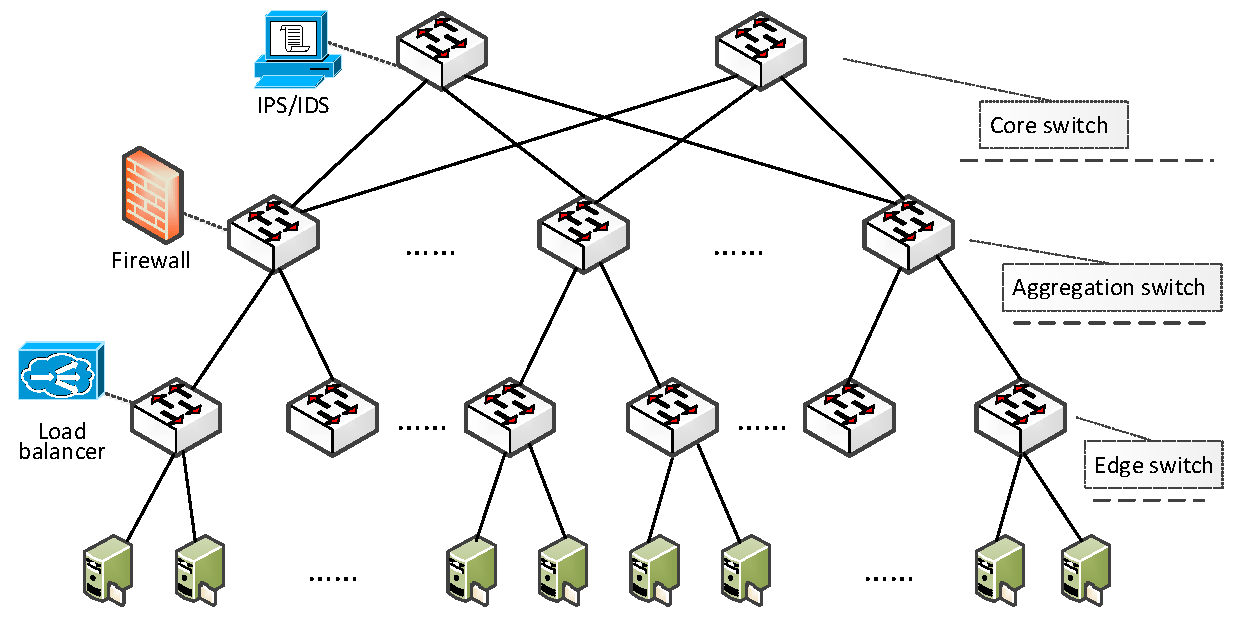
\includegraphics[width=3 in]{fig/topology.pdf}
	\caption{Datacenter network and hardware middlebox deployment}
	\label{fig:topo}
\end{figure}

% Our virtual middleboxes network placement algorithm also takes into consideration some realistic constraints in the physical machine. For example, with SR-IOV \cite{sriov} enabled host visualization, the traffic of VM is directly forwarded (through DMA) to the network interface card. Therefore, the VM-to-VM communication inside a host is bounded by the maximum switching capacity in the network interface card (NIC). Due to the speed limitation on hardware switching inside NIC, it can not be improved by either increasing the number of virtual functions or cores \cite{netvm}. Thus we need to consider such reliability constraint during virtual MBs placement.


To the best of our knowledge, we are the first to model the middlebox virtual network placement problem in multi-tenant datacenter networks with minimal performance guarantees. Extensive simulations on large-scale datacenter topology have shown the effectiveness of our VMs placement algorithm. The accept ratio approaches to 90\% with regard to a variety of tenants' requests in a large-scale datacenter topology. Compared with the greedy placement algorithm, our algorithm can also greatly reduce the fragment that can not be used by newly arrived tenant requests. Compared with the hardware middlebox placements in current datacenters, our VMs placement shows significant saving on network bandwidth but provides the performance guarantee. Generally, the lack of knowledge of the virtual middlebox network bandwidth consumptions has blocked the deployment of middleboxes as a service in datacenter, our study will be helpful to achieve a better understanding of this problem to build more flexible software-based cloud services.

%In general, we focus on tenant's requirement abstraction and effective VMs placement algorithm to achieve high network resource utilization in a datacenter. The contribution of this paper can be summarized as follows,
%\begin{itemize}
%	\item
%	\item the placement algorithm is effective and tested on our testbed.
%	\item moreover, we addressed the scalable issue of the mb placement which is the first time. because it is hard to evaluate the system requirement of mb, besides, the requirement is also variable.
%\end{itemize}

The rest of this paper is organized as follows. Sec. \ref{sec:background} reviews the background and related works on tenant's performance guarantee in the multi-tenant datacenter. Sec. \ref{sec:abstraction} describes our abstraction of middlebox and the communication model. The VMs placement algorithm is explained in Sec. \ref{sec:algorithm}, and the simulation based performance evaluation is demonstrated in Sec. \ref{sec:simulation}. Sec. \ref{sec:final} concludes this paper.

\section{Background and Related Works}\label{sec:background}
\textbf{Multi-tenant datacenter }
Large-scale datacenter is the core infrastructure for cloud based services. Datacenter network is organized in a multi-level tree-like topology. See Fig. \ref{fig:topo}, each rack typically contains 40+ servers, each of which is configured a 10Gbps network interface card (NIC) connecting to the top-of-the-rack (ToR) switch. The ToR switch will balance the traffic to multiple aggregation switches. All aggregation switches are further connected to the core switches. Note that the communication bandwidth between adjacent layers is oversubscribed by a ratio from 2:1 to 10:1, which may vary slightly with different configurations \cite{B13cta, williamson2010has}.

In multi-tenant data center environments, a tenant can rent multiple virtual machines (VMs) on physical servers. The VMs are configured with different amounts of CPUs, memories and storage resources. From the network perspective, we usually model the computation and storage resource to be the number of slots requested in physical machine. All VMs assigned to a tenant are interconnected to form a virtual network (VN) such that VMs can communicate with each other to exchange data. The traffic inside a multi-tenant datacenter carries external traffic to and from Internet, intra-tenant traffic between a tenant's application VMs and inter-tenant traffic. Specifically, the inter-tenant traffic consists of flows between tenants and flow between tenant and providers \cite{B13cta}, which can also be considered as a special tenant. Inter-tenant communication increases with the increase of services offered by cloud providers. Based on recent measurement in public cloud provider, 65\% of traffic happens between VMs belonging to one tenant VN and 35\% is among different VNs or tenant-provider communication \cite{B13cta, P13acs}.

\textbf{Middleboxes in multi-tenant datacenter }
Network functions are also necessary and provided in the form of hardware middleboxes in current datacenters.  However, hardware middelboxs are known to have several drawbacks. For example, working as a shared resource, the hardware middleboxes can only provide common services used by all tenants instead of providing customized tenant requests. Once the middlebox failed, all the tenants will be affected. Besides, the fixed locations of hardware middleboxes result in aggregated network bandwidth consumption and cause network congestion \cite{ClickOS, Y15NFV}. 

An alternative solution to hardware middleboxes is network function virtualization (NFV) \cite{NFV}. Deploying software middleboxes will greatly improve the flexibility, manageability and cost-efficiency. Software middlebox is not necessary to be shared and able to provide customized services with performance guarantee for each dedicated tenant. It has been shown that the software middleboxs are able to offer equivalent functionalists as the corresponding hardware implementation \cite{D12tpp, S12dai, G13dio, ClickOS}. The advance of software defined networking (SDN) further facilitates the deployment and management of software middlebox running in datacenters. Although there remains unsolved challenges before it can be integrated into the cloud ecosystem, the perspective of deploying flexible software middlebox for isolated tenants has motivated us to extend the previous works to realize predictable middlebox virtual networks through effective virtual middleboxes placement.


%SecondNet \cite{G10sad}, Seawall \cite{seawall}, Gatekeeper \cite{R11gsb}, Elastic Switch \cite{elasticswitch}, Oktopus \cite{B11tpd},
\textbf{Placement of services with performance guarantee}
Since the underlying network is shared by tenants, the application can be affected by variable and unpredictable network performance. A series of works have been proposed to enable traffic isolate and provide bandwidth guarantee, including Oktopus \cite{B11tpd}, FairCloud \cite{P12fst}, etc. The above works focus only on intra-tenant communication. The inter-tenant traffic isolation is addressed by Hadrian \cite{B13cta}. Through hierarchical hose model, the communication dependencies can be explicitly declared. The cloud provider then allocates resources according to the specification of tenants. 

Most of previous works only considered the bandwidth guarantee for applications. As far as we know, little work addresses the bandwidth guarantee for virtual MBs in multi-tenant datacenters \cite{7243304}. The NFV cloud computing platforms, like NFV OPEN LAB \cite{HuaweiNFV} and CloudNFV \cite{CloudNFV}, provide NFV management and orchestration as applications. Theoretically, to obtain effect use of resources, various NFV placement objectives have been studied, for example, remaining data rate, latency, number of used network node as well as distance and setup cost, see \cite{M14sap, cohen2015near} and the references therein. However, they could not provide bandwidth guarantee for tenants. Stratos \cite{stratos12} considered the middlebox placement in multi-tenant datacenters through a systematic way by avoiding network congestion. In contrast, we first study the bandwidth consumption problem of virtual middleboxes and then propose effective placement algorithm to make good use of network resources.

\section{Abstraction of Virtual Middlebox Network}\label{sec:abstraction}
In a multi-tenant datacenter, by leveraging the network function virtualization (NFV), cloud providers provide middlebox as a fundamental network service to tenants, like both computing and storage resources. A tenant could specify their middlebox and application (i.e., computation/storage) requirements in forms of VMs and the expected minimum bandwidth requirement for intra- and inter-tenant communication. Cloud providers will then assign VMs for middleboxes (in short, MB VMs) and applications (in short, APP VMs) according to the tenant's request. The cloud providers also enforce the middlebox policies, i.e., the sequence of middleboxes that a flow must traverse. In this section, we explain the model for APP VMs and MB VMs. We then introduce the abstraction of virtual networks associated to one tenant.


\subsection{Model of APP VMs}
To provide predictable network performance for the communication of $N$ APP VMs in one tenant, users typically specify the minimum bisection bandwidth $B^{in}$ for individual APP VM. Analogous to previous proposals \cite{B13cta, P12fst}, the requirement of the minimum bandwidth guarantee for each APP VM belonging to the same tenant can be abstracted by the \emph{hose model}. In the hose model (see the thick black arrows in Fig. \ref{fig:hose}, tenant P), the application VMs are connected to a logical switch by a link of capability $B^{in}$.

\begin{figure}
	\centering
		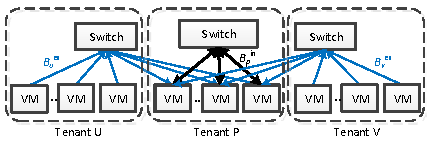
\includegraphics[width=3.5 in]{fig/tagmodel.pdf}
	\caption{Intra-tenant communication and inter-tenant communication}
	\label{fig:hose}
\end{figure}

Similarly, for the cross tenants communication, a tenant can specify the bandwidth request for a single APP VM. The minimum bandwidth guarantee for inter-tenant traffic of each APP VM is defined by $B^{ex}$. We extend the VN model of Hadrian \cite{B13cta} to support multiple external links. If the current tenant communicates to multiple tenants. The minimum bandwidth for each communication pair is guaranteed to be $B^{ex}$. The communication pattern between tenants can be expressed by a directed graph. We use the definition of \emph{communication dependency} in \cite{B13cta} to explicitly specify the peer-to-peer traffic pattern. A tenant with a dependency of \{*\} means that he could allow any other tenants' communication request. We call this kind of tenant open tenant while the tenant who has communication requests to open tenants are called client tenant. When the dependency is set as P:\{U, V\}, it means that the communication from tenant U and tenant V to tenant P are allowed. An example is illustrated in Fig. \ref{fig:hose}, the thin blue arrows show the communication between tenant U and tenant P, as well as tenant V and tenant P.

% Here is an example: i) A:\{B,C\}, ii) B:\{A\}, iii) C:\{*\}, which means that the communications between tenant A and tenant B, tenant A and tenant C are allowed. Therefore, the APP VMs' request of a tenant can be characterized by a four-tuple $<N, B^{in}, B^{ex}, dependencies>$.



\subsection{Model of MB VMs}\label{sec:modelformb}

Middleboxes perform different network functions to meet traffic demand of applications. A tenant may varies network functions simultaneously to process packets of different traffic class, as shown in Fig. \ref{fig:chain}. Each request consists of a sequence of various MBs, such as firewall (FW), intrusion detection system (IDS), load balancer (LB), redundancy elimination (RE) and NAT Proxy, etc., which provide functionality of access control and traffic engineering. 
% Notice that the software MBs are dedicated for each tenant. Due to the security and reliability, the assigned MBs will not be shared with other tenants based on the SLA requirement.  


Generally, the communication between MBs can be abstracted by a directed-acyclic graph (DAG), where the vertex represents the type of middleboxes and the arc indicates the traffic flow between them. The external traffic should pass through the specified middleboxes one by one according to the DAG. The sequence can not be violated. Otherwise, the expected functionality will be ruined. In addition, we assume that the traffic still keeps the same when multiple MBs are introduced. This is reasonable because the traffic is the minimum bandwidth guaranteed for both intra- and inter-tenant communication. The normal traffic could pass all the rule checking and will not be blocked by middbleboxes like FW or IDS. For those middelboxes, e.g., RE or LB, which change the traffic load, they are usually placed at the end of the DAG. The variation of traffic is specified by the proposed parameters of $B^{in}$ and $B^{ex}$ in the aforementioned APP VMs model.

\begin{figure}
	\centering
		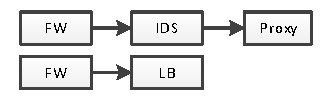
\includegraphics[width=3.0 in]{fig/chain.pdf}
	\caption{Abstraction of MBs: Two MBs chains}
	\label{fig:chain}
\end{figure}

% (important) However the abstraction of DAG may increase the representation and placement burden of middleboxes. Alternatively, the DAG can be simplified by partitioning the shared middleboxes to form multiple chains \cite{stratos12}. derived from the DAG given in Fig. \ref{fig:chain} (a) This operation is reasonable because a tenant can enable flow distribution at the head of DAG graph. , which classify the traffic 

Since a tenant may need to apply different middlebox policies to different traffic class. The tenant request can be classified into multiple MBs chains associated with different applications \cite{stratos12, M14sap, 7243304}. See Fig. \ref{fig:chain} as an example. The Internet traffic will pass Firewall, Intrusion Detection System and then NAT proxy. While the traffic from other tenant may only pass Firewall and Load Balancer. Therefore, a middlebox chain model can be defined by a tuple $\langle T, M \rangle$, where the type of MBs is denoted by a vector $T$, and the number of required MB VMs is denoted by a vector $M$. The direction of traffic flow is implicitly expressed by the sequence of items in the vector $T$. For instance, the first MB chain in Fig. \ref{fig:chain} can be expressed as $\langle T, M \rangle$, where $T=\{\text{FW, IDS, Proxy}\}, M=\{2, 4, 2\}$. It means that the tenant request for 2, 4 and 2 VMs of FW, IDS, and Proxy respectively. The traffic will arrive at FW first, and then go to IDS and pass Proxy before reaching the application VMs.

\subsection{Virtual Network Model} 
We combine the MB model and APP model together to form the virtual network (VN) model to represent the tenant's request. The interaction between VMs of the same tenant is expressed by the host model. The middlebox chain should be attached to the ingress path of the external link of the VN. Such that, all external traffic coming into APP VMs must traverse through these specified middlebox chains which provide access control and other network functions. CloudMirror \cite{cloudmirror} provided a new network abstraction that allows the applications to specify their directional and specific communication pattern. We adopt a cascade of \emph{Tenant Application Graph (TAG)} proposed in \cite{cloudmirror} to specify the VN model. 

Fig. \ref{fig:abstraction} (a) shows an example, where a sequence of MBs is attached at the external link of APP VMs of tenants. The arrow shows the traffic flow. Arrival traffic of tenant A will pass through all these middleboxes before being distributed to the application services. Similarly,  the departure traffic of tenant A is forwarded to its destination (tenant P) which needs to pass through the middleboxes of tenant P first \footnote{Some corporations may have the requirement to detect the departure traffic through additional middleboxes. We leave this for future work. }.  Fig. \ref{fig:abstraction} (b) uses the cascade of TAG model to abstract the communication dependency of VNs. The external traffic passing through each type of MB VMs in sequence are expressed by the dedicated directional arrows. The internal traffic of APP VMs is expressed by bi-directional arrows, each of which has a capacity of $B_{A}^{in}$ (tenant A) or $B_{P}^{in}$ (tenant P). The external traffic of each VM of tenant A (resp. tenant P) is bounded by $B_{A}^{ex}$ (resp. $B_{P}^{ex}$). 
\begin{figure}
	\centering
		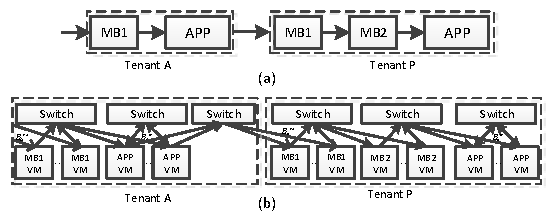
\includegraphics[width=3.5 in]{fig/abstraction.pdf}
	\caption{Virtual Network Model. (a) the communication between two tenants; (b) cascade of TAG}
	\label{fig:abstraction}
\end{figure}

% and 3) the traffic from the other VN belonging to the same tenant
In general, two kinds of traffic may go through the MBs before come to the Application VMs, 1) the Internet traffic; 2) the traffic from other tenant. When declaring a connectivity relationship, this external link can only communicate with those specified VNs. The unauthorized traffic will be blocked by MBs. Based on the models of APP VMs and MB VMs, a tenant can specify the connectivity of an external link which receives (or sends) traffic from any VN. In summary, a tenant's request can be specified by multiple virtual networks (VNs) and each VN can be specified by a tuple $<N, B^{in}, B^{ex}, dependencies, T, M>$. 

\noindent \textbf{Remark } 
It is a remarkable fact that the behavior of current software middleboxes is actually not easy to predict in the real system. The performance depends on multiple factors, including workload like traffic demands, type and number of rules, and middelbox design, e.g., algorithm design, systematical implementation, etc. Therefore, the scalability of MBs is important and need to be considered by the cloud service provider. Once the virtual network are placed in datacenter, it is hard to find a proper resource to migrate MBs and re-allocate live flows across MBs with performance guarantee \cite{G13dio}. We discuss the scalability issue in Appendix.

% Specifically, the VMs inside the blue dotted line are pre-allocated VMs for middleboxes subrequirement, which are shared by both types of middleboxes requests. If there are scale-out or failover request, specified MBs will be placed on these VMs to provide performance guarantee. 

\section{Virtual Network Placement}\label{sec:algorithm}
Based on the tenant's request, the cloud provider allocates enough resource for MBs and APPs. The VMs request will be satisfied by providing enough free slots on physical machines (PMs). The network function demand consists not only the bandwidth request but also the capability to process a specific class of traffic in order. The placement strategy is realized by a logically centralized controller, which manages datacenter operations through a global view of the network topology. SDN based traffic engineering manipulates the underlying network routers to explicitly direct the class of traffic through each middlebox sequentially. If there are not sufficient resource, the request will be rejected. 


The virtual machine placement problem has attracted a lot of attentions recently, which can be formalized as a multi-dimensional packing problem with various constraints. This problem is proved to be NP-hard \cite{packing, fischer2013virtual}. Therefore we search for effective heuristic solution to maximize the datacenter resources utilization. Before introducing the VMs placement algorithm, we first explain some practical constraints in our design.

\begin{figure}
	\centering
		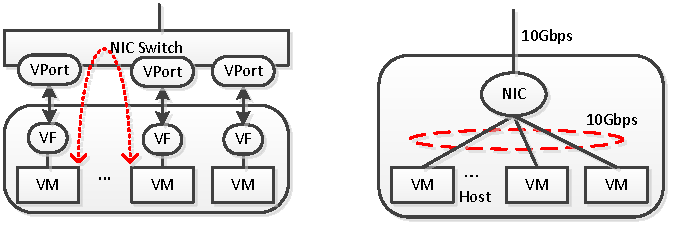
\includegraphics[width=3.5 in]{fig/nic.pdf}
	\caption{Bandwidth constraint of NIC in PM}
	\label{fig:nic}
\end{figure}

\subsection{Bandwidth Constraint within a Physical Machine}

Existing operating systems typically copy the data from user space to kernel space and then move the data to the buffer of NIC. The data copies cause a long delay during packet transmission. Recent works allows applications to access the NIC card directly without involving kernel processing which direct DMA to and from a VM, like Single Root I/O Virtualization (SR-IOV) \cite{sriov}. Intel SR-IOV allows multiple VMs to access the NIC through L2 address. Most data center networks have enable the SR-IOV in their system to accelerate the data processing\footnote{Virtual Ethernet Port Aggregator (VEPA) forwards packets out of the host and come back via an external switch to be transmitted to a VM. Since VEPA will cost more network resource, we do not consider this situation in this paper.}. When using SR-IOV, packets are switched on a per-port basis in the NIC between VMs on a shared port, as that shown in Fig. \ref{fig:nic}. The hypervisor configures the NIC switch on the SR-IOV network adaptor to provide network connectivity to the VMs. However, the communication between VMs is bounded by the NIC switch capacity. NetVM \cite{netvm} tried to overcome this limitation by providing  memory sharing without passing through the NIC. However, due to some problems like the potential security thread in multi-tenant datacenter, this new feature is not applied in current commodity environment yet. In general, the bandwidth constraint inside PM can be expressed that the traffic between VMs of the same PM is bounded by a maximum bandwidth, see the model at the right side of Fig. \ref{fig:nic}. We need to take this constraint into consideration during VMs placement algorithm design.


\subsection{VM Placement Strategies}\label{sec:placement}

%Given virtual middlebox network request, the middleboxes and applications should be carefully placed into the datacenter. Otherwise, it may cause severe waste of resources. For example, one native placement is shown Fig. \ref{fig:careless}. Assume there are three type of MiddleBox VMs. The first type $MB_{1}$ is placed in the same subtree with App VMs while the other two types are placed on another subtree. In this case, the traffic to the APP VMs have to pass the links under the switch twice to go through all MiddleBox VMs. A refined placement is to place the last type of MiddleBox VMs as close as possible to the APP VMs. For instance, after placing the App VMs, the $MB_{3}$ is placed first, then the $MB_{2}$ and the $MB_{1}$ is placed afterward.


In the subsequence, we analyze the bandwidth consumption of various approaches to achieve a better understanding of the MBs placement problem. Given a virtual network request, and suppose that we have found several candidate subtrees that have enough slots to hold the required VMs, people can find out two primary strategies to distribute VMs among the subtrees. One approach is to always place all kinds of MB VMs in the same subtree with the corresponding APP VMs in a predefined ratio $R=N/\sum_{i} M{i}$, where $M_{i}$ is number of $i^{th}$ MBs in vector $M$. That is, given the number of MB VMs, the maximum number of APPs that can be served. Each partition contains sufficient MBs to serve the APPs and thus can work independently. We call such an approach ``TRAIN", since it works like a train consisting multiple cars of MBs. As shown in Fig. \ref{fig:train}, it consists of three groups horizontally, each of which can process all arrival traffic to the APP VMs in the same group. Another approach is to make the same kind of middleboxes as a group and place them together in the subtree. We call this approach ``TRUCK" since it works like a truck to take cargo of the same kind. As shown in Fig. \ref{fig:truck}, MB$_{1}$, MB$_{2}$ and APP are divided first and put to subtree separately.

% TRAIN divides the APP VMs and MB VMs together by following a certain proportion. Each partition is placed in a subtree. Fig. \ref{fig:train} describes this strategy. The APP VMs are divided into three parts, APP$_{1}$, APP$_{2}$ and APP$_{3}$. Meanwhile, each kind of MiddleBox is divided into three parts to serve the corresponding parts of APP VMs. For example, MB$_{11}$ and MB2$_{21}$ only serve the arrival traffic of $APP_{1}$. The division of the APP VMs is determined by the available resources (slots and bandwidth) in the subtrees. After dividing the App VMs, we can compute the number of MiddleBox VMs $VM^{i}_{MB}$ in subtree $i$ by $VM^{i}_{MB} = \lceil \frac{VM^{i}_{App}}{VM_{App}}*VM_{MB}\rceil$. Since $\lceil \frac{VM^{i}_{App}}{VM_{App}}*VM_{MB}\rceil \geq \frac{VM^{i}_{App}}{VM_{App}}*VM_{MB}$, thus $\sum_{i=1}^{N_{l}}{VM^{i}_{MB}} \geq VM_{MB}$, where $N_{l}$ is the number of subtrees of link $l$. Note that TRAIN allocates more MiddleBox VMs than what the tenant's request. TRUCK places all APP VMs in one subtree while the MB VMs in another subtrees, as depicted in Fig. \ref{fig:intuition} (b). In this case, the expected bandwidth of tenant on link of the subtree is $a=N\cdot B^{ex}$.   

% Therefore, the second strategy may waste CPU resources if the integer number of MBs is required.

% However, the first strategy needs to find a subtree that can accommodate all App VMs of the tenant. If there is no such subtrees, the first strategy cannot work. The second strategy is able to place VMs into the subtrees with small fragments.

We analyze the bandwidth cost of these two strategies, as that illustrated in Fig. \ref{fig:intuition}. Assume the arrival traffic is $a$, the traffic flow is illustrated in thick blue arrow. It will first pass through the MB VMs and then reach the APP VMs. See Fig. \ref{fig:intuition} (a), by using the approach TRAIN, the arrival traffic to the left node is $\frac{MB_{l}}{MB} a$ where $MB_{l}$ denotes the number of MBs at the leaf node and $MB$ denotes the total number of MBs. Similar, the traffic to the right side is $\frac{MB_{r}}{MB} a$, where $MB_{l}+MB_{r}=MB$.The communication for intra-tenant communication is 
\[
	\min(MB_{l}, MB_{r})RB^{in}
\]
which stems from the maximum flows between VMs belonging to the same tenant. In summary, the total down-stream bandwidth cost of the approach TRAIN is
\[
  a+2\min(MB_l, MB_r)RB^{in} 
\]
and the total upstream bandwidth cost of TRAIN in \ref{fig:intuition} (a) is
\[
 2\min(MB_l, MB_r)RB^{in}
\]

We then analyze the bandwidth cost from the simple scenario of VMs placement with regard to the approach TRUCK, where all MBs are placed in one side and all APPs are placed in another side. As illustrated in Fig. \ref{fig:intuition} (b), we can easily achieve the bandwidth cost on both links. In short, the total bandwidth cost of the approach TRUCK is
\[
 a \text{ (upstream)} \quad \text{and}  \quad 2a \text{ (downstream)}
\]

\begin{figure}
  \centering
  \subfigure[TRAIN: dividing virtual middleboxes network horizontally]{
    \label{fig:train} %% label for 2 subfigure
    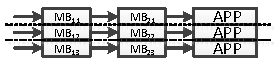
\includegraphics[width=3.0 in]{fig/train.pdf}}
  \subfigure[TRUCK: dividing virtual middleboxes network vertically.]{
    \label{fig:truck}%% label for 1 subfigure
    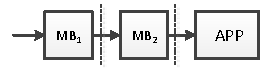
\includegraphics[width=3.0 in]{fig/truck.pdf}}
		\caption{Two partition strategies to distribute the VMs among subtrees}
\end{figure}

\begin{figure}
	\centering
		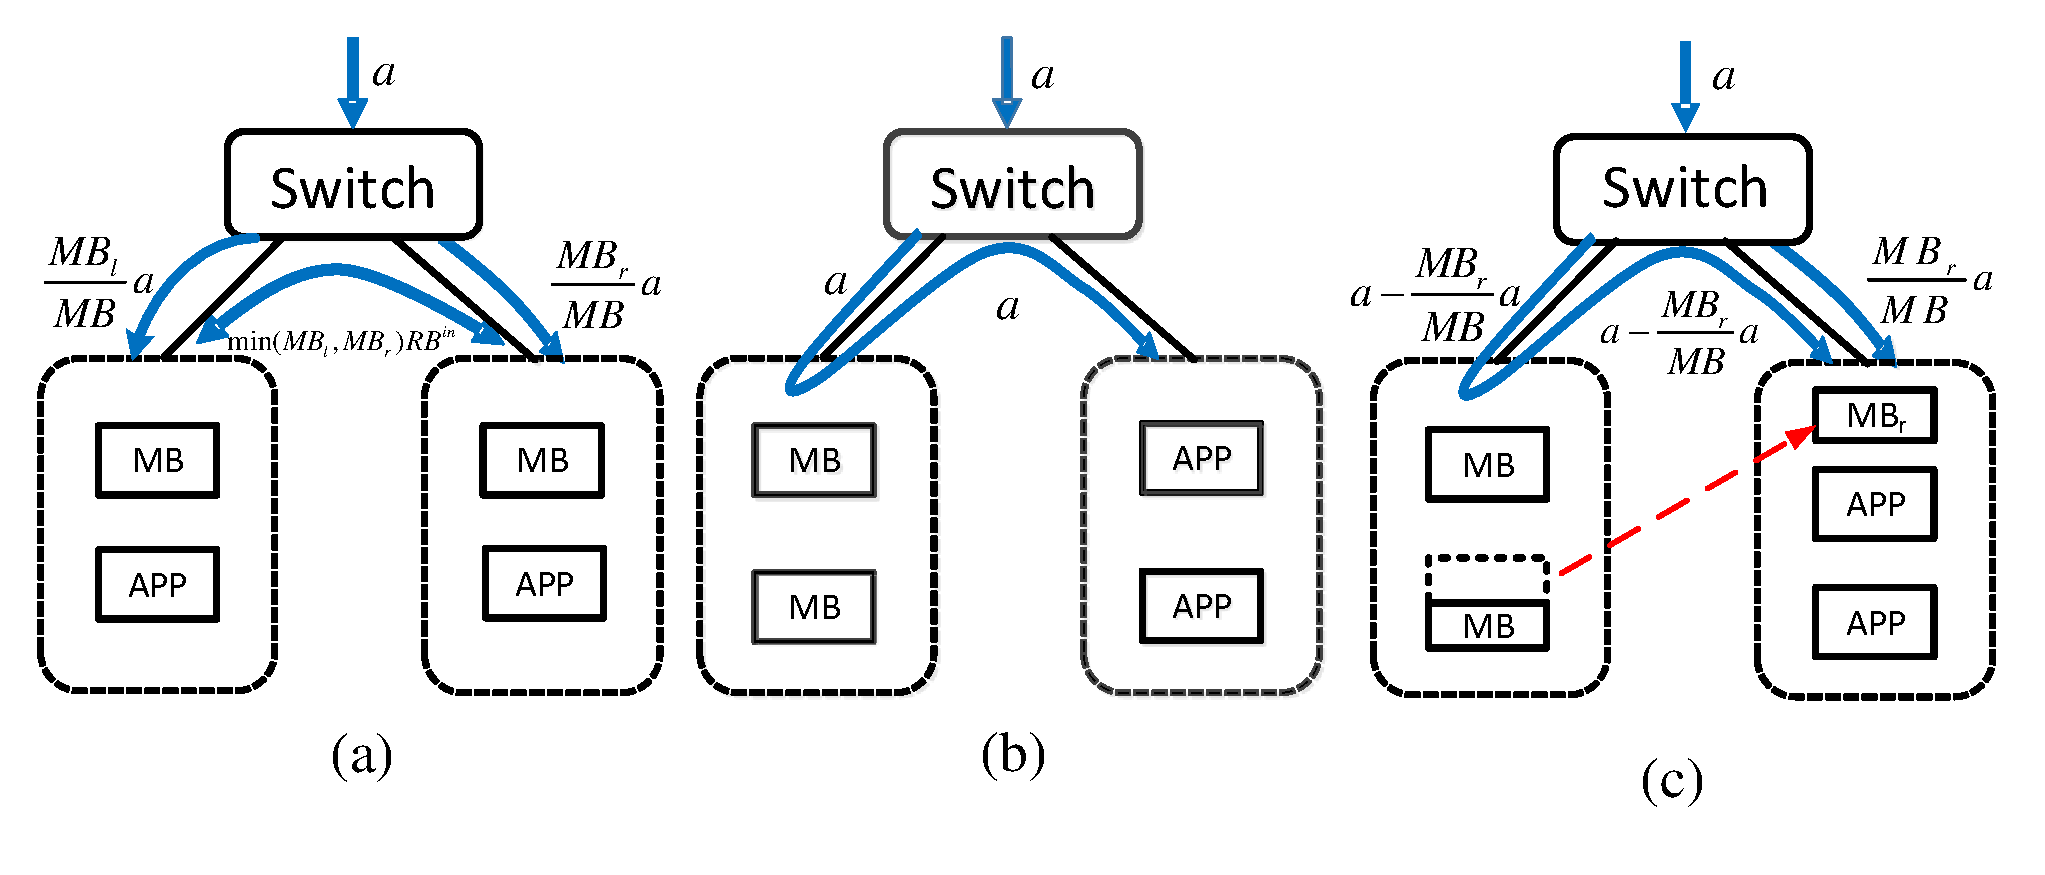
\includegraphics[width=4 in]{fig/intuition.pdf}
	\caption{Illustration of placement algorithm}
	\label{fig:intuition}
\end{figure} 

Based on above results, we further show that in what kind of scenarios, the bandwidth consumption can be reduced by revising the placement strategy. We move part of MBs in form of chain from left leaf to the right. Denote the amount of MBs at right side by $MB_{r}$ and the total number of MBs by $MB$. The bandwidth cost is shown in Fig. \ref{fig:intuition} (c), where the amount of traffic is split proportionally due to the movement of MBs. Notice that the sum of flows going to the right side is $a$ since all APPs is placed there. However, the traffic on the left link reduces from $a$ to $a-\frac{MB_{r}}{MB}a$ compared with the placement given in Fig. \ref{fig:intuition} (b). Therefore, we know that the bandwidth cost can be decreased by co-location of APP and MB sub-chain.
\begin{figure}
	\centering
		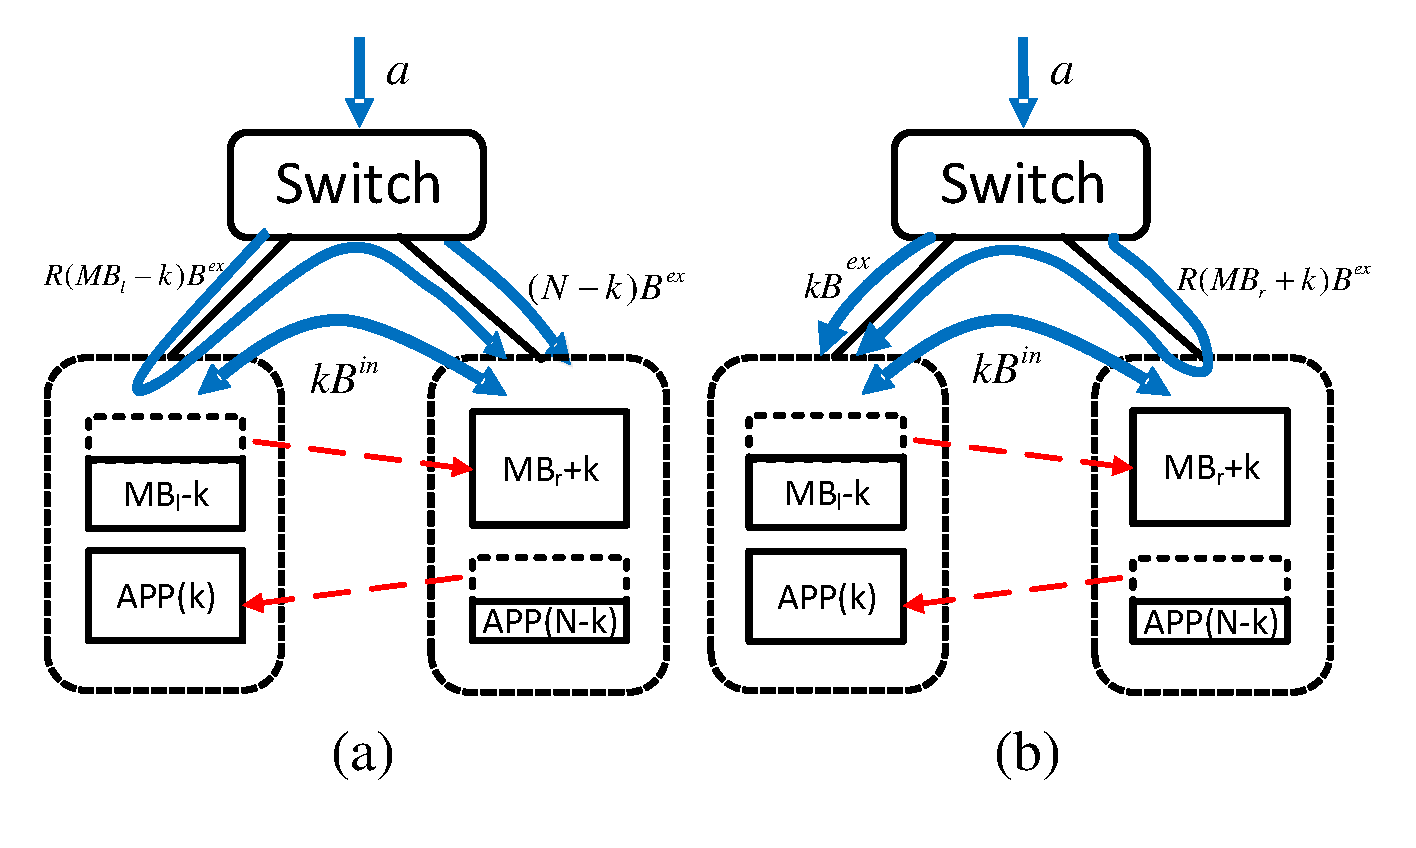
\includegraphics[width=3.5 in]{fig/intuition2.pdf}
	\caption{Illustration of VMs placement by exchanging $k$ MB VMs on the left leaf with $k$ APP VMs on the right leaf. $APP(k)$ denotes $k$ APP VMs here. }
	\label{fig:intuition2}
\end{figure} 

Although we have a co-location suggestion when seeing free slots in one machine, we still do not know which placement algorithm is better, TRAIN or TRUCK? or can we get more benefit by using a combination of these two algorithms? To address this challenge, we explore to further reduce the bandwidth cost by exchanging $k$ APPs on the right leaf with $k$ MBs on left leaf in Fig. \ref{fig:intuition} (c). The process is shown in Fig. \ref{fig:intuition2} which consists of two cases. When $k$ is small, MBs on the left side is sufficient to serve the associated $k$ APPs in the same leaf. The extra MBs should serve the APPs on the right side. So there are flows from left to the right side on the link, see Fig. \ref{fig:intuition2} (a). On the other hand, with the increasing of $k$, MBs on the left leaf will not be sufficient to serve the APPs on the same leaf. The flow goes in the reverse direction, see Fig. \ref{fig:intuition2} (b). 

We then analyze the bandwidth cost on the above scenario. Let $MB_l$ be the number of MBs on the left subtree in Fig. \ref{fig:intuition} (c), and $MB_r$ be the number of MBs on the right subtree. Without loss of generality, we consider that $k$ is not larger than half of the number of APPs. Therefore, we have 
\begin{equation}
a = NB^{ex}, \qquad R(MB_l+MB_r) = N, and \quad k\leq \frac{N}{2}
\end{equation}
where $N$ is the number of APP VMs, while $R$ is a predefined ratio in Sec. \ref{sec:placement}.  We consider both the uplink and downlink bandwidth in our analysis.

\textbf{Case 1. } ($MB_l-k$)MBs is sufficient to serve the associated $k$ APPs on the left leaf, as illustrated in Fig. \ref{fig:intuition2} (a).

We considering the variation of uplink or downlink bandwidth on Fig. \ref{fig:intuition2} (a) and Fig. \ref{fig:intuition} (c). Since the ($MB_l-k$)MBs is sufficient to serve the associated $k$ APPs, the extra MBs on the left leaf serve the APPs on the right. Hence, there are extra flows from left to right.

Let $\omega_l$($\omega_r$) and $\omega_l^{'}$($\omega_r^{'}$) denote the downlink bandwidth cost on left(right) link before and after the exchange of $k$ VMs, respectively. The variation of downlink bandwidth on left(right) link is:
%When considering the variation of the downlink bandwidth before and after the exchange of the $k$ APPs, denoted by $\omega_l$ and $\omega_l^{'}$ respectively, we have

\begin{equation}
\begin{aligned}
\Delta \omega_l &= \omega_l^{'} - \omega_l\\
&=R(MB_l-k)B^{ex}+kB^{in}-R\cdot MB_l\cdot B^{ex} \\
&= k(B^{in}-RB^{ex}) \\
\Delta \omega_r &= \omega_r^{'} - \omega_r \\
&=(N-k)B^{ex}+kB^{in}-NB^{ex} \\
&=k(B^{in}-B^{ex})
\end{aligned}
\end{equation}

Similarly, the variation of uplink bandwidth on left(right) link is:
\begin{equation}
\begin{aligned}
\Delta \omega_l &= \omega_l^{'} - \omega_l\\
&=R(MB_l-k)B^{ex}-kB^{ex}+kB^{in}-R\cdot MB_l\cdot B^{ex} \\
&= kB^{in}-kB^{ex}-RkB^{ex} \\
\Delta \omega_r &= \omega_r^{'} - \omega_r = kB^{in}
\end{aligned}
\end{equation}

To calculate the variation of bandwidth consumption, we add $\Delta \omega_l$ and $\Delta \omega_r$. In uplink and downlink cases, we have the same result
\begin{equation}
\begin{aligned}
\Delta \omega &=\Delta \omega_l +\Delta \omega_r = k(2B^{in}-(R+1)B^{ex})
\end{aligned}
\end{equation}

Hence, we can tell that when $2B^{in} > (R+1)B^{ex}$, $\Delta \omega > 0$, the bandwidth consumption increases after exchange, TRUCK performs better than TRAIN. Otherwise, TRAIN get a better performance.

\textbf{Case 2. } ($MB_l-k$)MBs is not sufficient to serve the associated $k$ APPs on the left leaf, as illustrated in Fig. \ref{fig:intuition2} (b). 

We consider the variation of uplink or downlink bandwidth on Fig. \ref{fig:intuition2} (b) and Fig. \ref{fig:intuition} (c). Since the ($MB_l-k$)MBs is not sufficient to serve the associated $k$ APPs, there are extra flows from right to left.

In this case, we have the following constraints:

\begin{equation}
\begin{aligned}\label{equ:constraint2}
R(MB_l-k) < k \Longrightarrow R\cdot MB_l < k(R+1)
\end{aligned}
\end{equation}

The variation of downlink bandwidth on left(right) link is:

\begin{equation}
\begin{aligned}
\Delta \omega_l &= \omega_l^{'} - \omega_l=kB^{ex}+kB^{in} - R\cdot MB_l \cdot B^{ex} \\
\Delta \omega_r &= \omega_r^{'} - \omega_r=R(MB_r+k)B^{ex}+kB^{in} - NB^{ex} 
\end{aligned}
\end{equation}

When considering the variation of the uplink bandwidth, the variation of uplink bandwidth on left(right) link is:

\begin{equation}
\begin{aligned}
\Delta \omega_l &= \omega_l^{'} - \omega_l= kB^{in}-R\cdot MB_l\cdot B^{ex} \\
\Delta \omega_r &= \omega_r^{'} - \omega_r\\
&= R(MB_r+k)B^{ex}-(N-k)B^{ex}+kB^{in}
\end{aligned}
\end{equation}

To calculate the variation of bandwidth consumption, we add $\Delta \omega_l$ and $\Delta \omega_r$. Eq. (\ref{equ:constraint2}) is used when calculate the upper bound. In uplink and downlink cases, we have the same result:

\begin{equation}
\begin{aligned}
\Delta \omega &=\Delta \omega_l +\Delta \omega_r \\
&= 2kB^{in}+kB^{ex}-NB^{ex}-R\cdot MB_l\cdot B^{ex}\\
&\quad+R(MB_r+k)B^{ex} \\
&= 2kB^{in}+kB^{ex}-(N-R\cdot MB_r)B^{ex}-R\cdot MB_lB^{ex}\\
&\quad+kRB^{ex} \\
&= 2kB^{in}+k(R+1)B^{ex}-2R\cdot MB_lB^{ex} \\
&< k(2B^{in}-(1+R)B^{ex})
\end{aligned}
\end{equation}

The upper bound of $\Delta \omega$ equals to the result in case1. Hence, the same result is obtained. When $2B^{in} > (R+1)B^{ex}$, TRUCK performs better than TRAIN. Otherwise, TRAIN get a better performance.

% Based on the above observation, we design an effective but simple algorithm call ``MISSILE'' for virtual middleboxes network placement in multi-tenant datacenters.
\subsection{VM Placement Algorithm}
Based on the insight into two strawman solutions, namely TRAIN and TRUCK, we proposed a more powerful algorithm, MISSILE, to offer predicable network performance to each tenant while minimizing bandwidth consumption and server resource wastes. The basic idea of our algorithm is to place the APP VMs and the MB VMs chain sequentially. The algorithm traverses the topology in a depth-first fashion to find candidate sub-tree to accommodate the VMs required by new tenant. Then we put APP VMs and MB VMs in the subtree according to the approach TRUCK or TRAIN based on the tenant's $B^{in}$, $B^{ex}$, and $R$. 

The detail of the algorithm is explained as follows. The algorithm is described in $Placement$, which takes a tenant request $t$ as input. Firstly, we need to find a lowest subtree with enough slots for $t$ in our topology using $FindLowestSubtree$ (line 2). The search starts from the server level and moves upward. When we have found a subtree, we place $t$ in it with $Alloc$ (line 4) and then check if there is enough bandwidth for $t$. If the placement fails because of the lack of slot or bandwidth, we find another subtree in the same level or upper level if there is no subtree in the same level.

$Alloc$ (line 22) is a function which takes a tenant request $t$, its APP and MB VMs' number and a subtree root as input. The function first checks if $root$ is a server: if so, it places $N_{app}$ and $N_{mb}$, and then returns. If $root$ is a higer level node, a judgement will decide whether we should use TRAIN or TRUCK to place APP VMs and MB VMs, and then we include the two basic placement algorithms. Both algorithms traverse the subtrees of the root and try to fill the subtrees with $N_{app}$ APP VMs and $N_{mb}$ MB VMs. For TRUCK, we place APP VMs first and then place MB VMs. But for TRAIN, we carefully choose the number of APP VMs and MB VMs so that MBs is sufficient for APPs in each subtree. Since all of the inter-tenant communication flows need to travel through the MiddleBox VMs, $AllocMB$ tries to place  a single type of MiddleBox VMs in a single physical machine to save the link's bandwidth in TRUCK but place all types of MBs in a single physical machine in TRAIN. In addition, the MiddleBox VMs are placed as close as possible to the corresponding App VMs to minimize the extra bandwidth between MiddleBox VMs and App VMs.

\begin{algorithm}[!htbp]
\caption{VM Placement Algorithm}
\label{alg1}
	\begin{algorithmic}[1]
	\Function {Placement}{Tenant t}
		\State st = FindLowestSubtree(t, 0)
		\While{$st != CORE$}
			\State	Alloc(t, t.appvm, t.mb, st)
			\If {t.success and ReserveBWtry}
				\State	ReserveBW
				\State  return true
			\EndIf
		\State st = st.next
		\If {st == NULL}
			\State FindLowestSubtree(t, level(st) + 1)
		\EndIf
		\EndWhile
		\State\Return{$false$}
	\EndFunction
	\State
	\Function {FindLowestSubtree}{$t, layer$}
		\For{$i \in layer$}
			\If{checkslot(t, i)}
				\For{$j \in child(i)$}
					\If{checkslot(t, j)}
						\State\Return FindLowestSubtree($t, layer-1$)
					\EndIf
				\EndFor
				\State\Return i
			\EndIf
		\EndFor
		\State\Return{FindLowestSubtree(t, layer+1)}
	\EndFunction
	\State
	\Function {Alloc}{$t, N_{app}, N_{mb}, root$}
		\If{root == PM}
			\State $placeAPP(t, N_{app}, root)$
			\State $placeMB(t, N_{mb}, root)$
			\If{$t.appvm==0$ and $t.mb==0$}
				\State t.success = true
			\EndIf
		\Else
			\If{$2B^{in} > (R+1)B^{ex}$}
				\State TRUCK($t, N_{app}, N_{mb}, root$)
			\Else
				\State TRAIN($t, N_{app}, N_{mb}, root$)			
			\EndIf
		\EndIf
	\EndFunction
	\end{algorithmic}
\end{algorithm}

%\textbf{Algorithm Complexity: } Since our algorithm recurses over a 3-level hierarchical datacenter structure. We....


%\subsection{Bandwidth Constraint within a Physical Machine:Example}
%For example, assume that each PM has 8 slots, while the internal bandwidth capacity of the NIC is $2B^{min}$. A tenant requests 4 VMs and the requested minimum bandwidth is $B^{min}$. The strategy of Hadrian will place the 4 VMs in a single VM, the internal bandwidth in the PM will be exhausted, illustrated in Fig. \ref{fig:example2}. There are four free slots available in the PM but they can not be allocated to other tenants. A careful placement that place one VM in a subtree while three VMs in another subtree. With this placement, neither the internal bandwidth nor the slots in the two PMs are exhausted.


\section{Performance Evaluation}\label{sec:simulation}
We evaluate our placement algorithm via simulation. A tree-like 3-level network topology, which is inspired by a real cloud datacenter with 70,000+ VMs, 40 physical servers with 10Gbps NICs, is assigned to a ToR switch. Each PM contains 16 slots. The oversubscribion at Tor is 2.5:1 and aggregation switch is 4:1. The over-subscription ratio are 4:1 at the leaf level and 10:1 at the spine layer.

To simulate tenant requests, we model the intra-tenant bandwidth $B^{in}$ to follow uniform distribution in the interval $[500, 1000]$Mbps, while $B^{ex}$ follows uniform distribution in $[200, 300]$Mbps. The number of APP VMs is randomly selected in $[5, 15]$. And the number of MBs is achieved based on the APP VM - MiddleBox Ratio $R$ randomly selected in $[2, 8]$. The type of MBs is randomly selected in $[1,4]$. The fraction of open tenants is set to be 10\% while the fraction of client tenants is set to be 25\%. Furthermore, there are also some tenants that have communication request with each other. We set the fraction of these tenants to be 15\%. For each test, we run 100 experiments and report the average results. In our simulation, tenant requests arrive continuously until the datacenter could not accept tenant request any more.

We consider three placement algorithms: (i) TRUCK that places the APP VMs and the MB VMs separately; (ii) TRAIN that places the APP VMs uniformly; (iii) MISSILE which places the APP VMs given in Algorithm 1. The reason that we only compare MISSILE with TRAIN and TRUCK is because previous studies could not be applied in our scenario. The most related work on virtual MBs placement proposed by Stratos \cite{stratos12} is not relevant for our problem setting due to two reasons: (1) they only consider the inter-tenant communication without addressing the APP VMs; and (2) the requests from multiple tenants are placed simultaneously in \cite{stratos12}, while we are able to place the request of arrival tenant one by one.

Fig. \ref{fig:blankslot} shows the waste slot distribution among servers with three placement algorithms. Obviously, the number of servers with wasting slots decreases with the increasing of the number of wasting slots per server in any of the three method. It is observable that there are 16 servers wasting 1 slots with TRAIN and TRUCK while MISSILE only have 8 servers that waste 1 slots. In general, TRAIN or TRUCK methods waste more than 2 times of slots comparing with MISSILE. More specifically, MISSILE tries to place the tenant request as long as there is a server with blank slots and tries to fill that server. On the other hand, TRUCK or TRAIN take a part of a server at one time, and may produce large amount of fragments that are hard to be used by newly arriving tenants in the future.

\begin{figure}
\center
    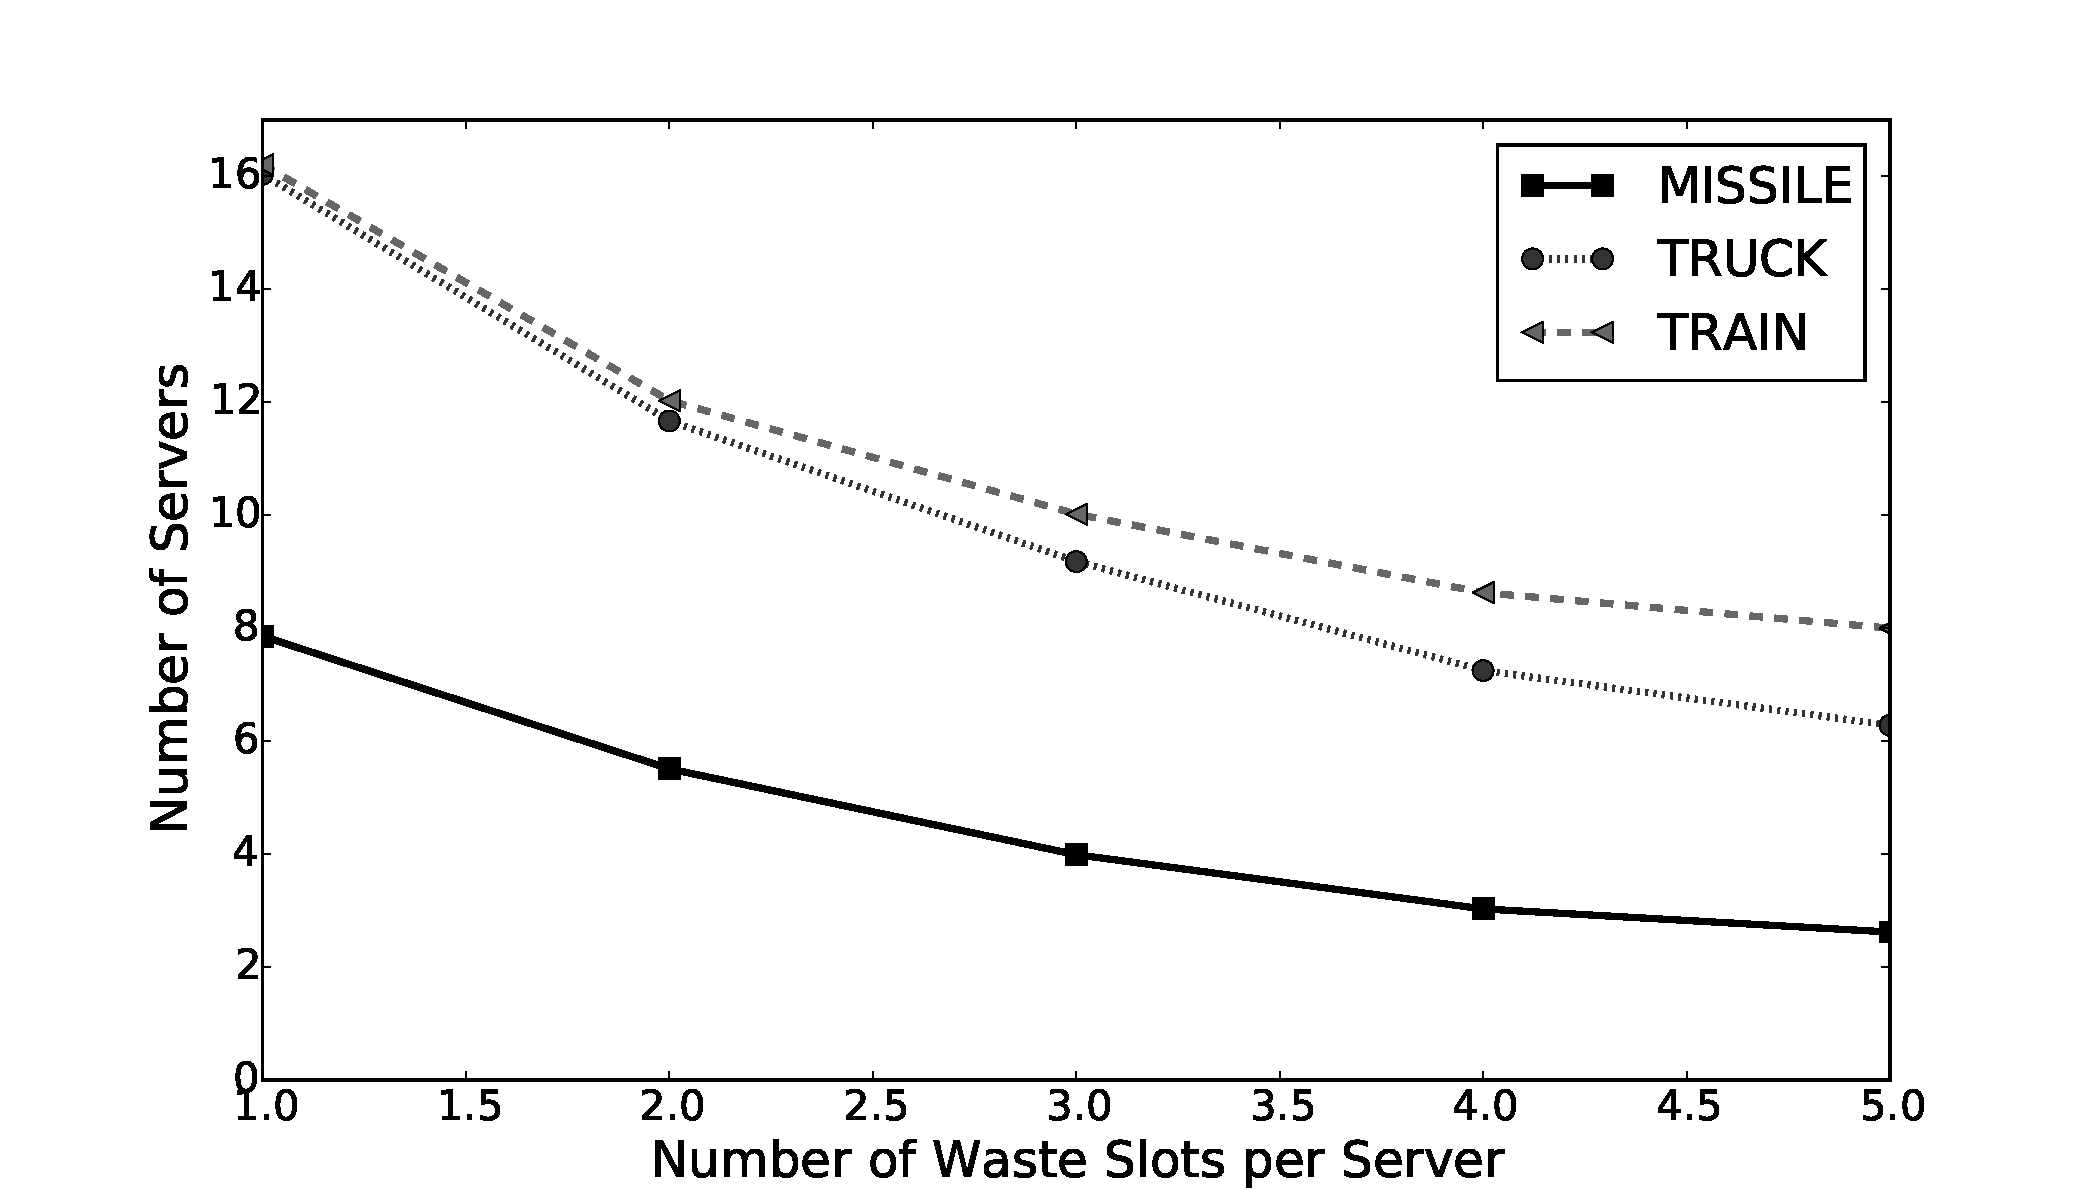
\includegraphics[width=2.8 in]{fig/BlankSlot.pdf}
    \caption{Waste slot distribution among servers}
    \label{fig:blankslot}
\end{figure}
\begin{figure}
  \centering
  \subfigure[Low bandwidth utilization distribution among servers]{
    \label{fig:blankbw_upload}%% label for 1 subfigure
    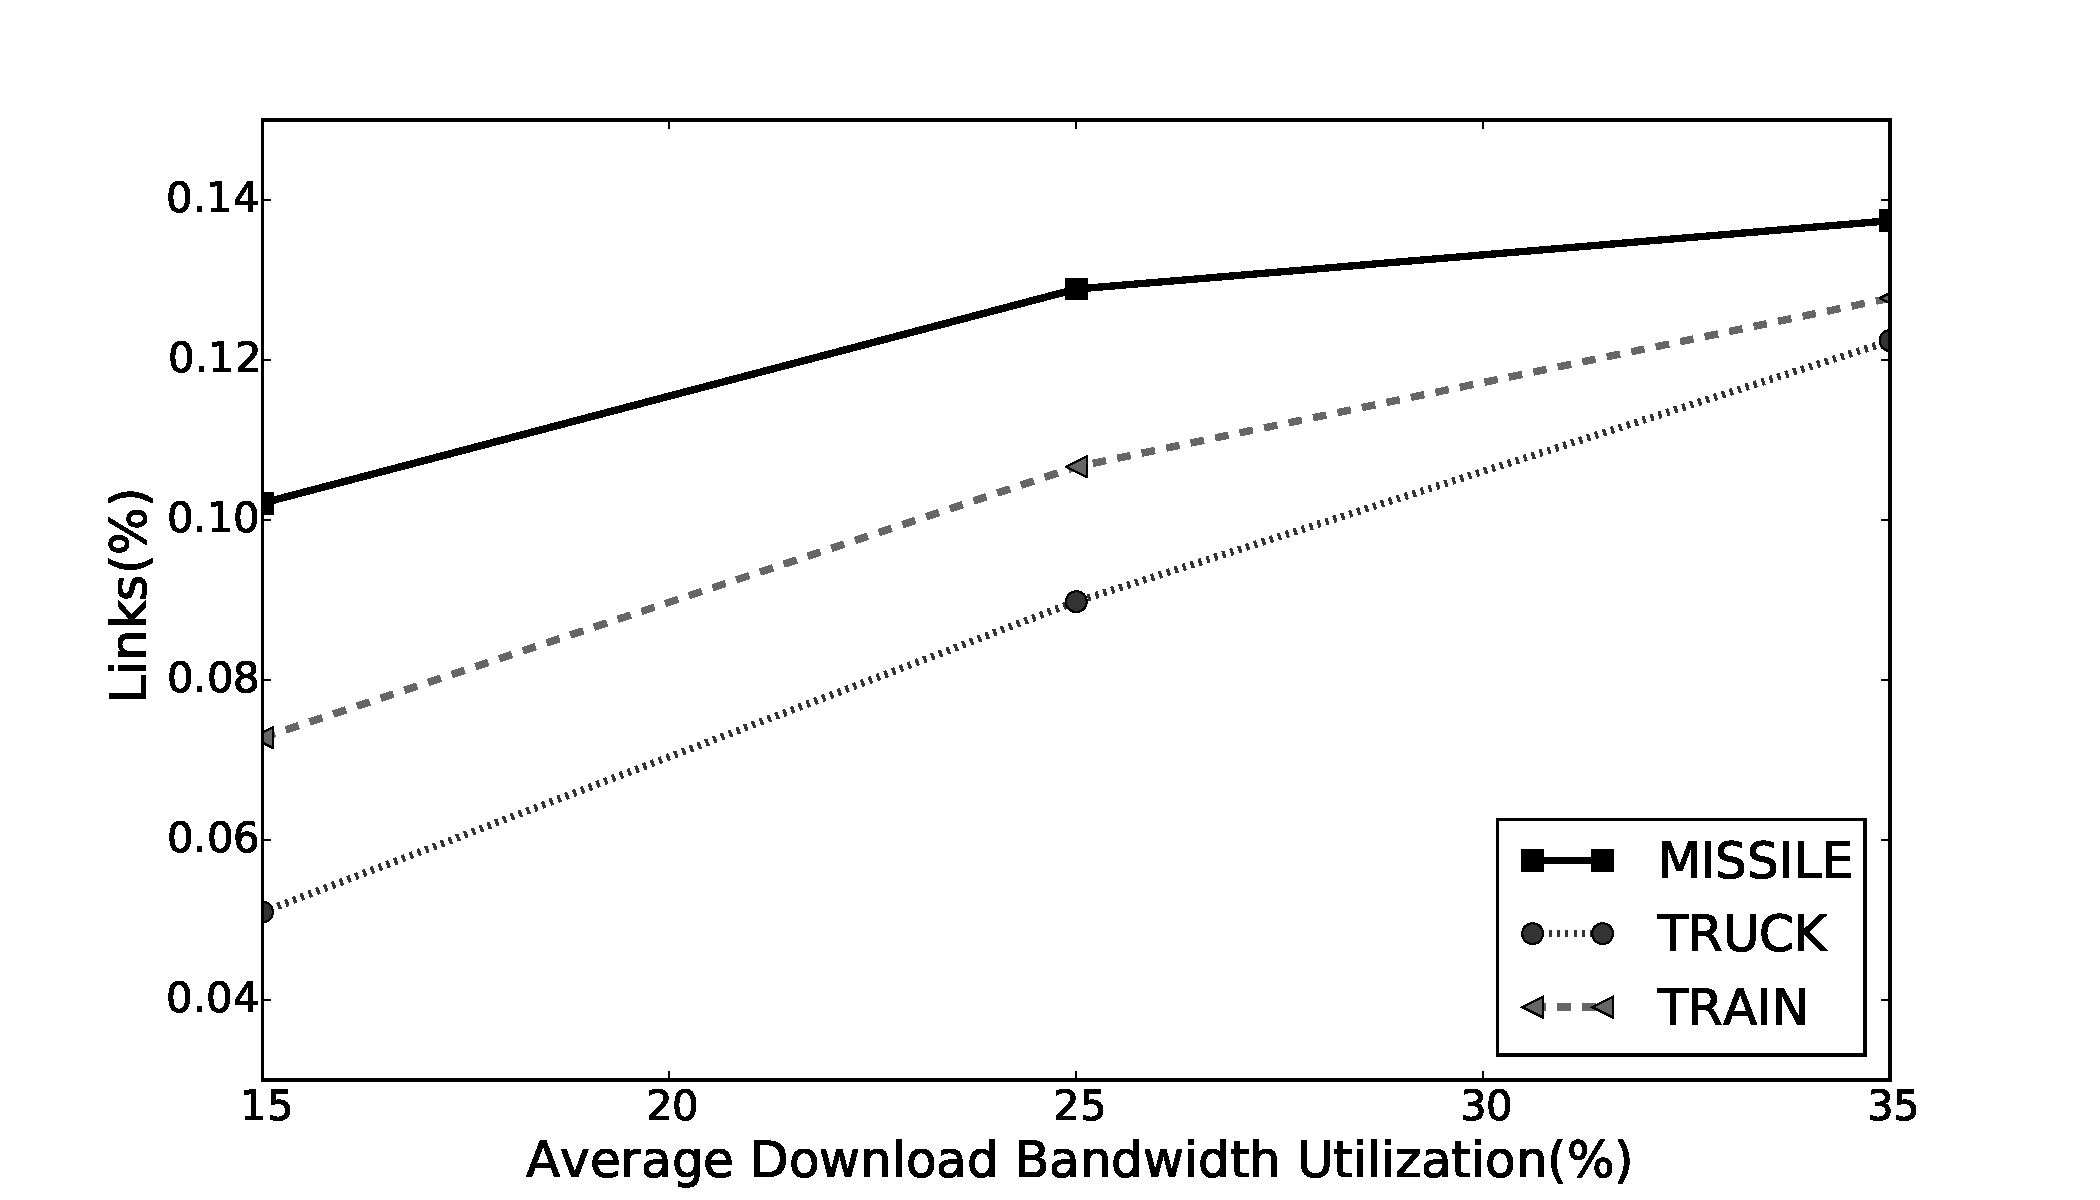
\includegraphics[width=2.8 in]{fig/BWUtil_low.pdf}}
  \subfigure[High bandwidth utilization distribution among servers]{
    \label{fig:blankbw_download} %% label for 2 subfigure
    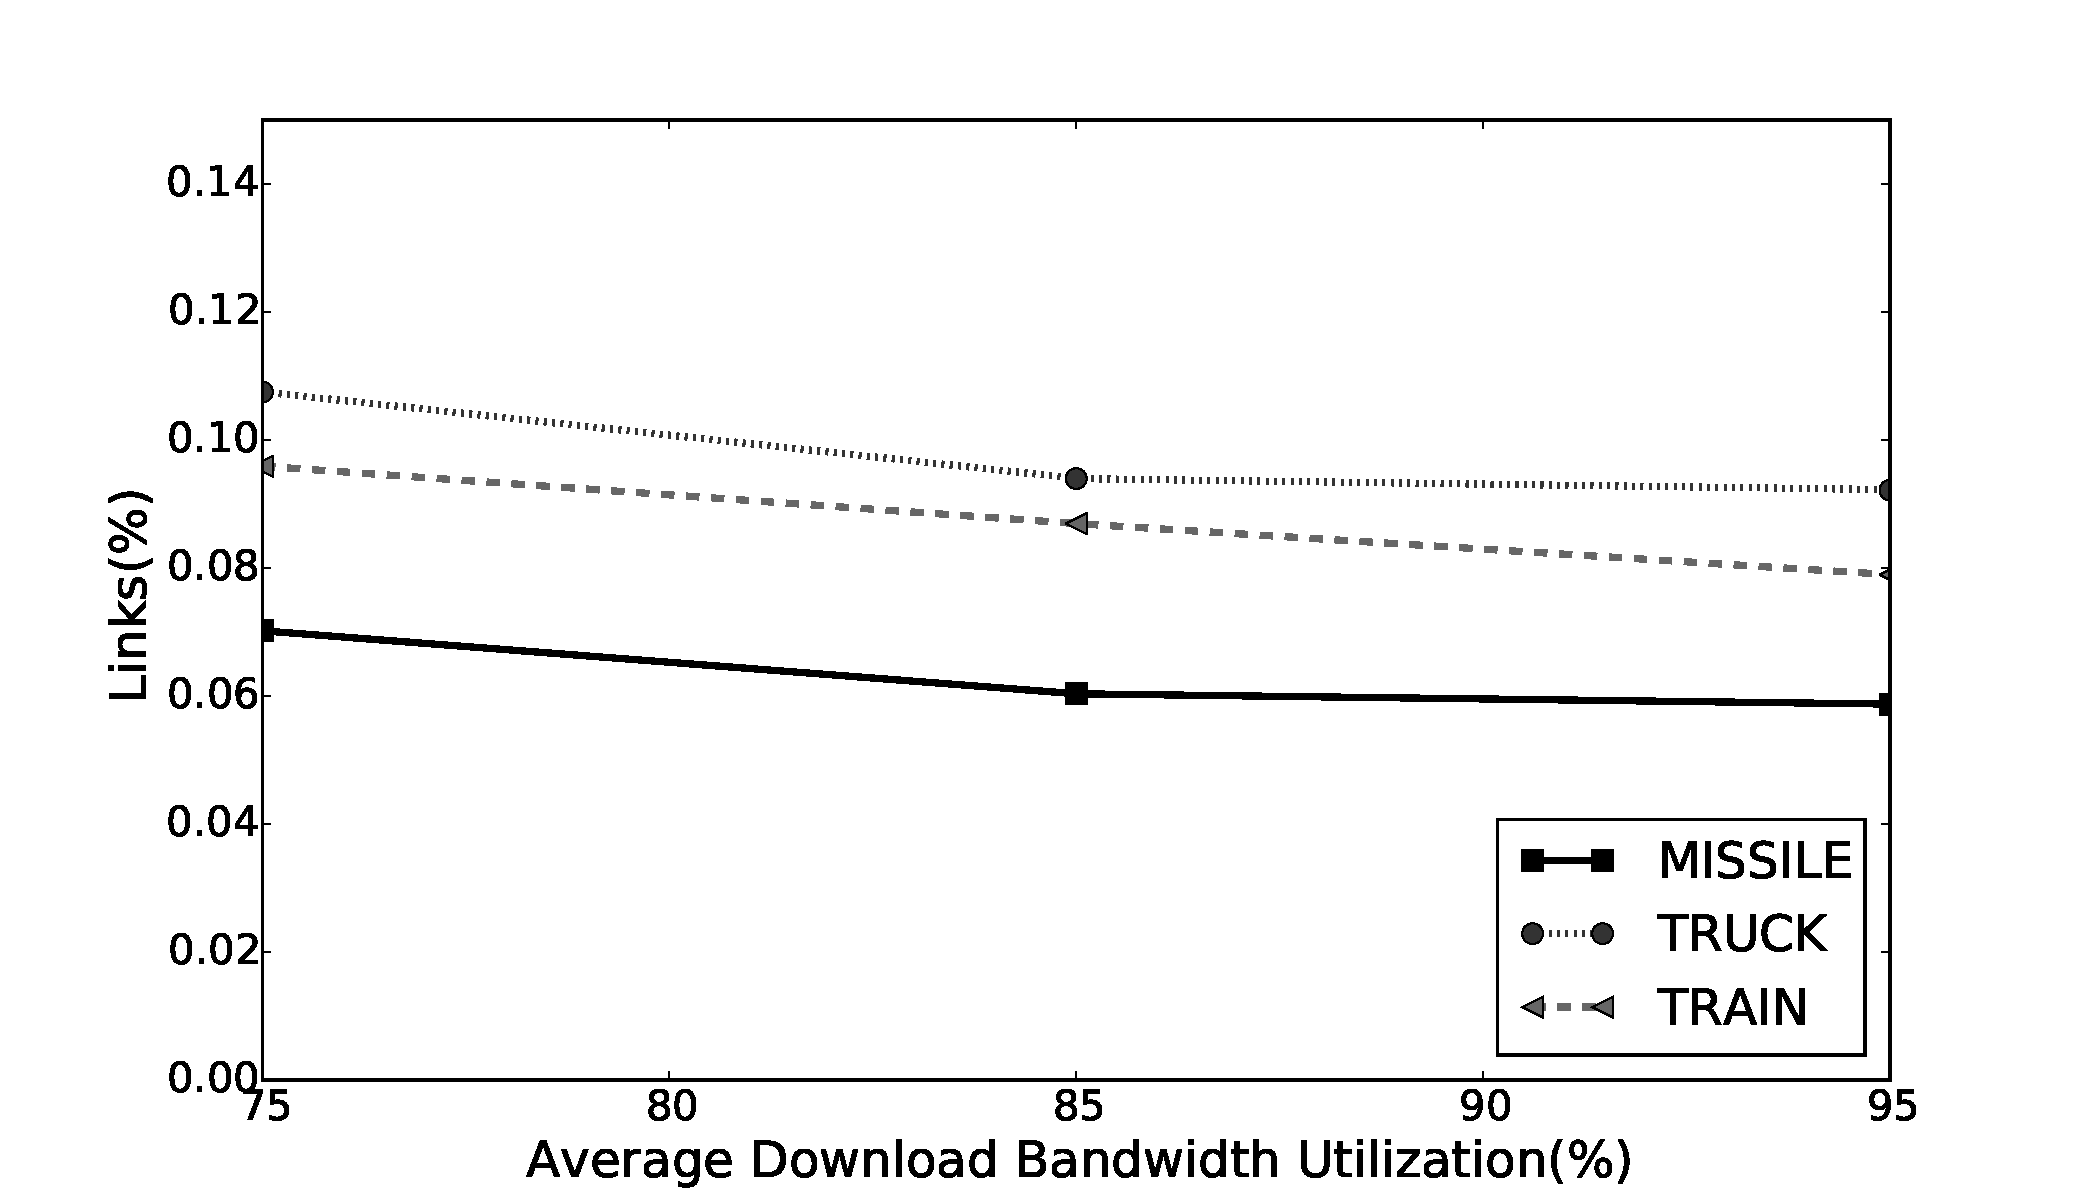
\includegraphics[width=2.8 in]{fig/BWUtil_high.pdf}}
    \caption{Bandwidth utilization distribution among servers}
    \label{fig:blankbw}
\end{figure}

In the next experiment, we evaluate the uplink bandwidth utilization of servers. Since the servers are on the same layer of the 3-level network topology, if there is one upload bandwidth consumption, there must have another download bandwidth consumption correspondingly. This lead to the result that the upload and download results are similar to each other. Hence, we just show the result of the download bandwidth here. The results are shown in Fig. \ref{fig:blankbw}, where the x-axis shows the average download bandwidth consumption, and the y-axis shows the percentage of the servers' uplinks. Fig. \ref{fig:blankbw}(a) shows the result when download bandwidth utilization is low. We can see that MISSILE has more links of this kind of bandwidth utilization than TRAIN or TRUCK. On the other hand, MISSILE has less links of high bandwidth utilization than TRAIN or TRUCK which is shown in \ref{fig:blankbw}(b). To sum up, MISSILE saves bandwidth efficiently while making a better use of PMs by contrast with Fig. \ref{fig:blankslot}.

We then evaluate the accept rate of tenants' requests under three mentioned placement algorithms. The result is shown in Fig. \ref{fig:acc_rate}. We take the average value of $B^{in}$ as x-axis and observe the accept rate. Here, average $B^{in}$ of 1100Mbps means that the tenants' $B^{in}$ follows the uniform distribution in $[1000, 1200]$Mbps. Obviously, MISSILE always accept more tenant requests than TRAIN or TRUCK. Even with large value of average-$B^{in}$, we still obtain good performance with MISSILE. 

Another observation of Fig. \ref{fig:acc_rate} is that the accept rate of TRUCK decreases rapidly with the increasing of average $B^{in}$. We explain this phenomenon in Fig. \ref{fig:acc_rate_boxplot}. With the box plot, we can see that TRUCK performed unsteadily in the 100 experiments when average $B^{in}$=1400Mbps: the accept rate may be under 35\% or exceed 65\%.

\begin{figure}
\center
    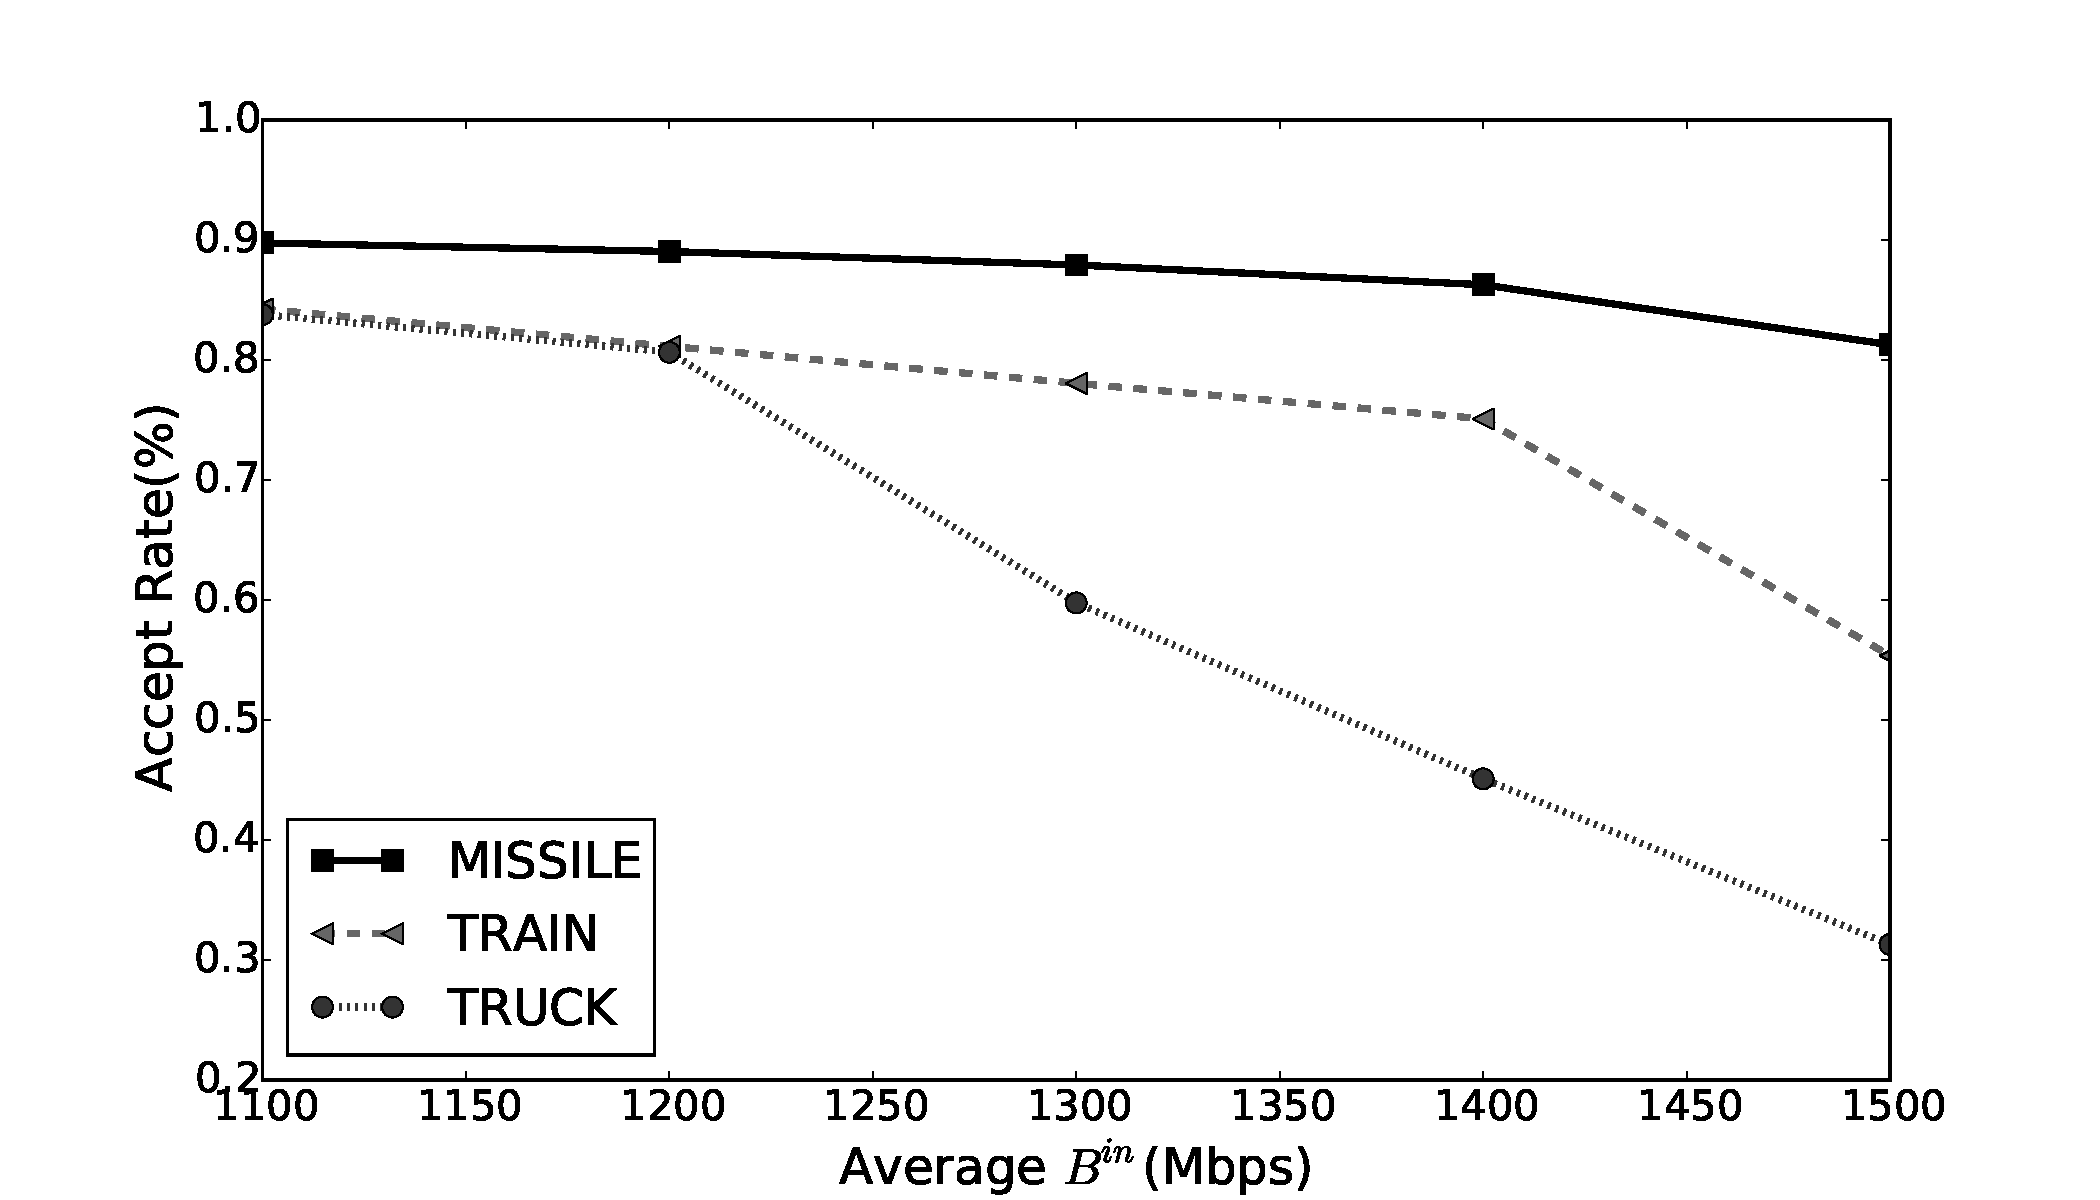
\includegraphics[width=2.8 in]{fig/acc_util.pdf}
    \caption{Accept rate under different $B^{in}$}
    \label{fig:acc_rate}
\end{figure}

\begin{figure}
\center
    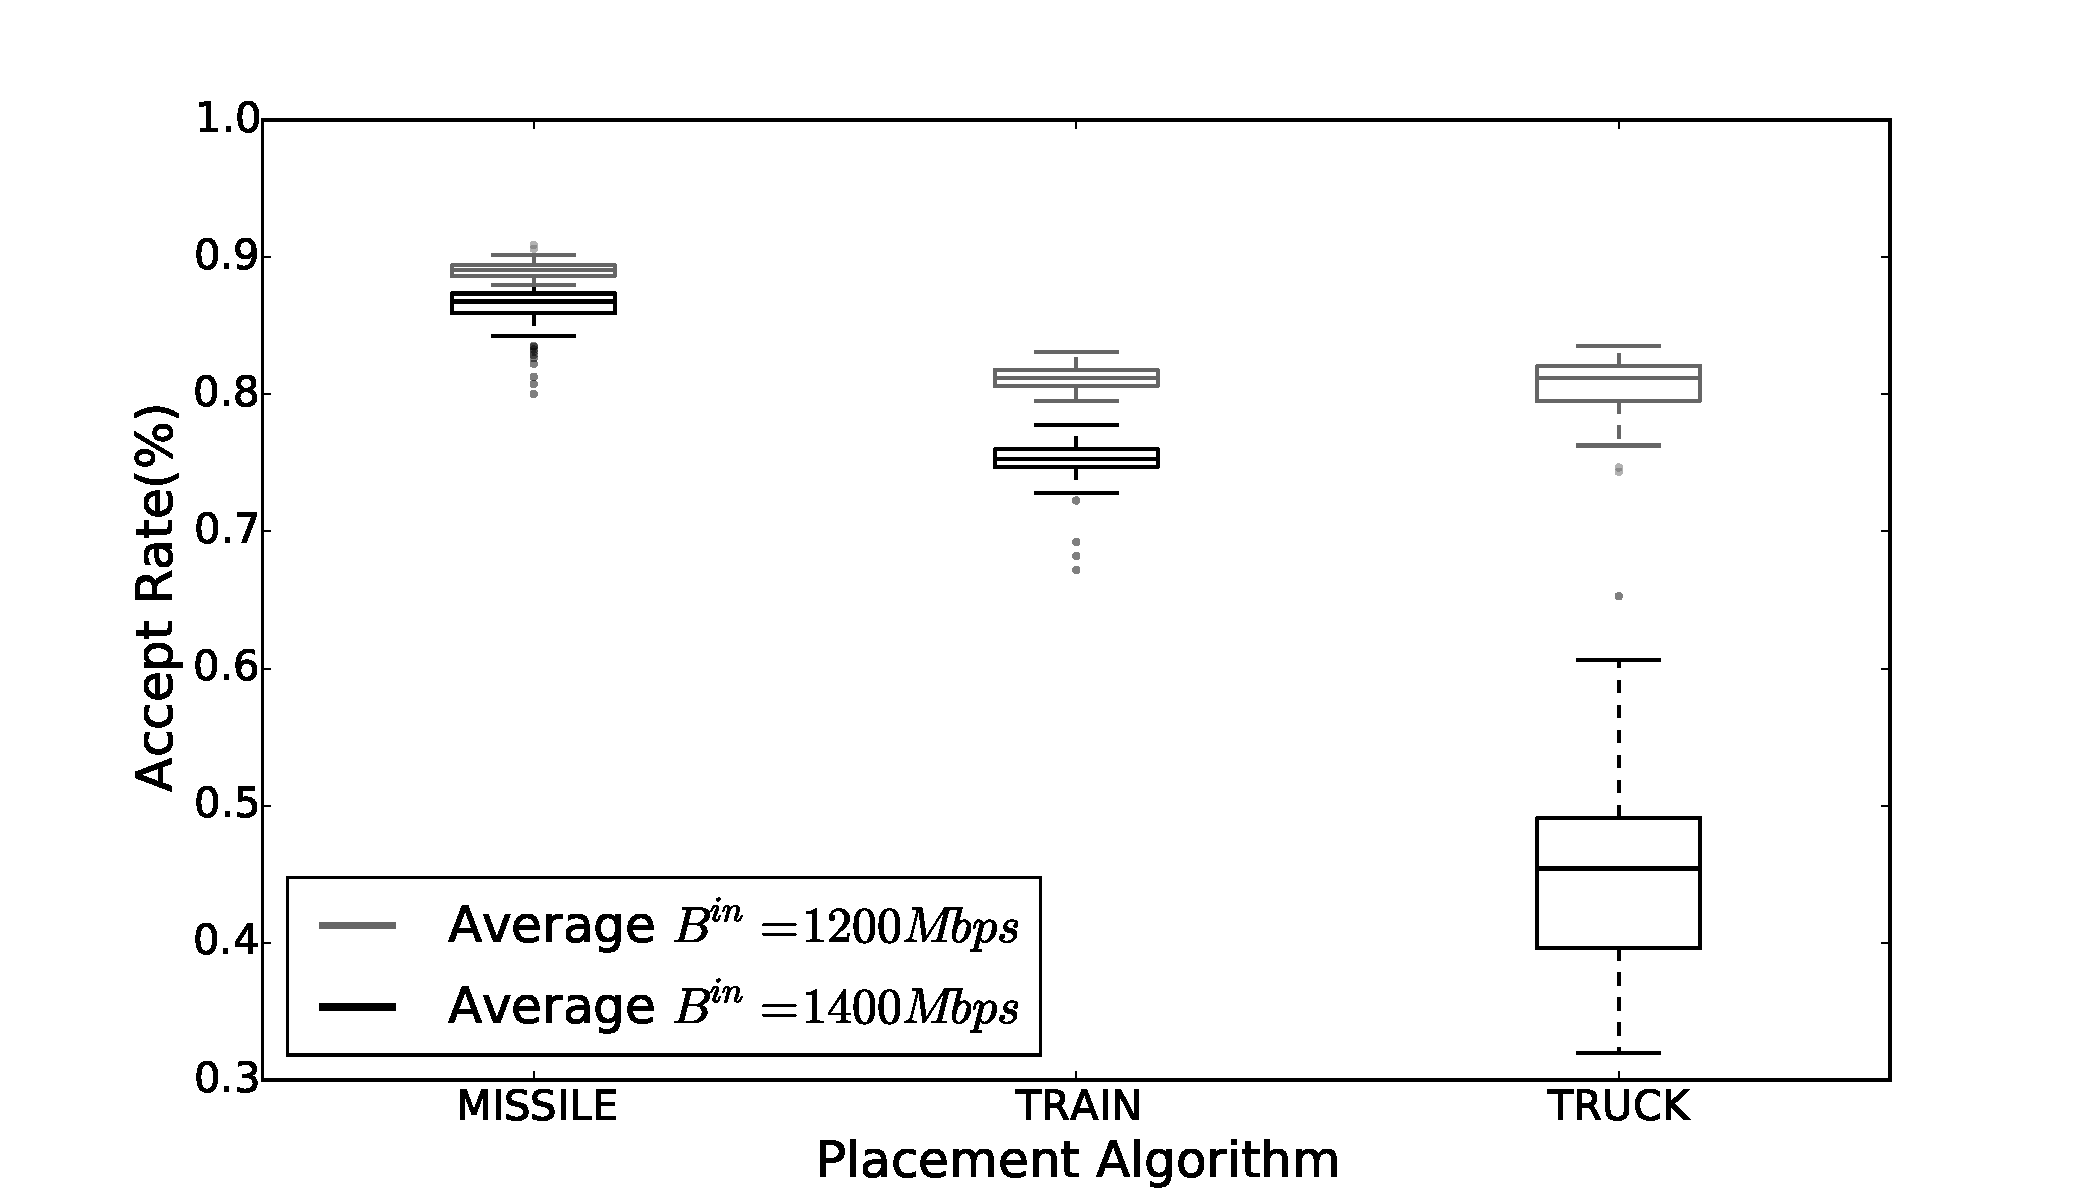
\includegraphics[width=2.8 in]{fig/accbox1400_1200.pdf}
    \caption{Accept rate under different Placement Algorithms}
    \label{fig:acc_rate_boxplot}
\end{figure}


We try to identify the impact of $B^{in}$ and bandwidth constraint inside a PM. We change the intra-tenant bandwidth $B^{in}$ to follow uniform distributions in different ranges. The inner physical machine limits the number of VMs allowed to be placed. The experimental results are shown in Fig. \ref{fig:constr}, where average-$B^{in}$ takes the value of $x$ (e.g. $500$) if it follows the uniform distribution in $[x-100, x+100]$ (e.g. $[400, 600]$). It is observable that when internal bandwidth constraint is considered, the accept rate of tenant request quickly drops while average-$B^{in}$ increases. This is because the internal constraint limits the location of VMs of new tenants. For example, host A with 16-slot capacity has placed 8 application VMs of tenant P, when tenant Q which is dependent on P comes, placing 8 application VMs again may produce bandwidth requirement $4 \times B_P^{in}+4 \times B_Q^{in}+B^{ex}$, and may exceed the internal bandwidth upper limitation. As a result, only 6 VMs of tenant Q is allowed to be placed into host A, the remaining two slots are then not available, which reduces the utilization of VM slots and increases the rejection rate dramatically.


\begin{figure}
\center
    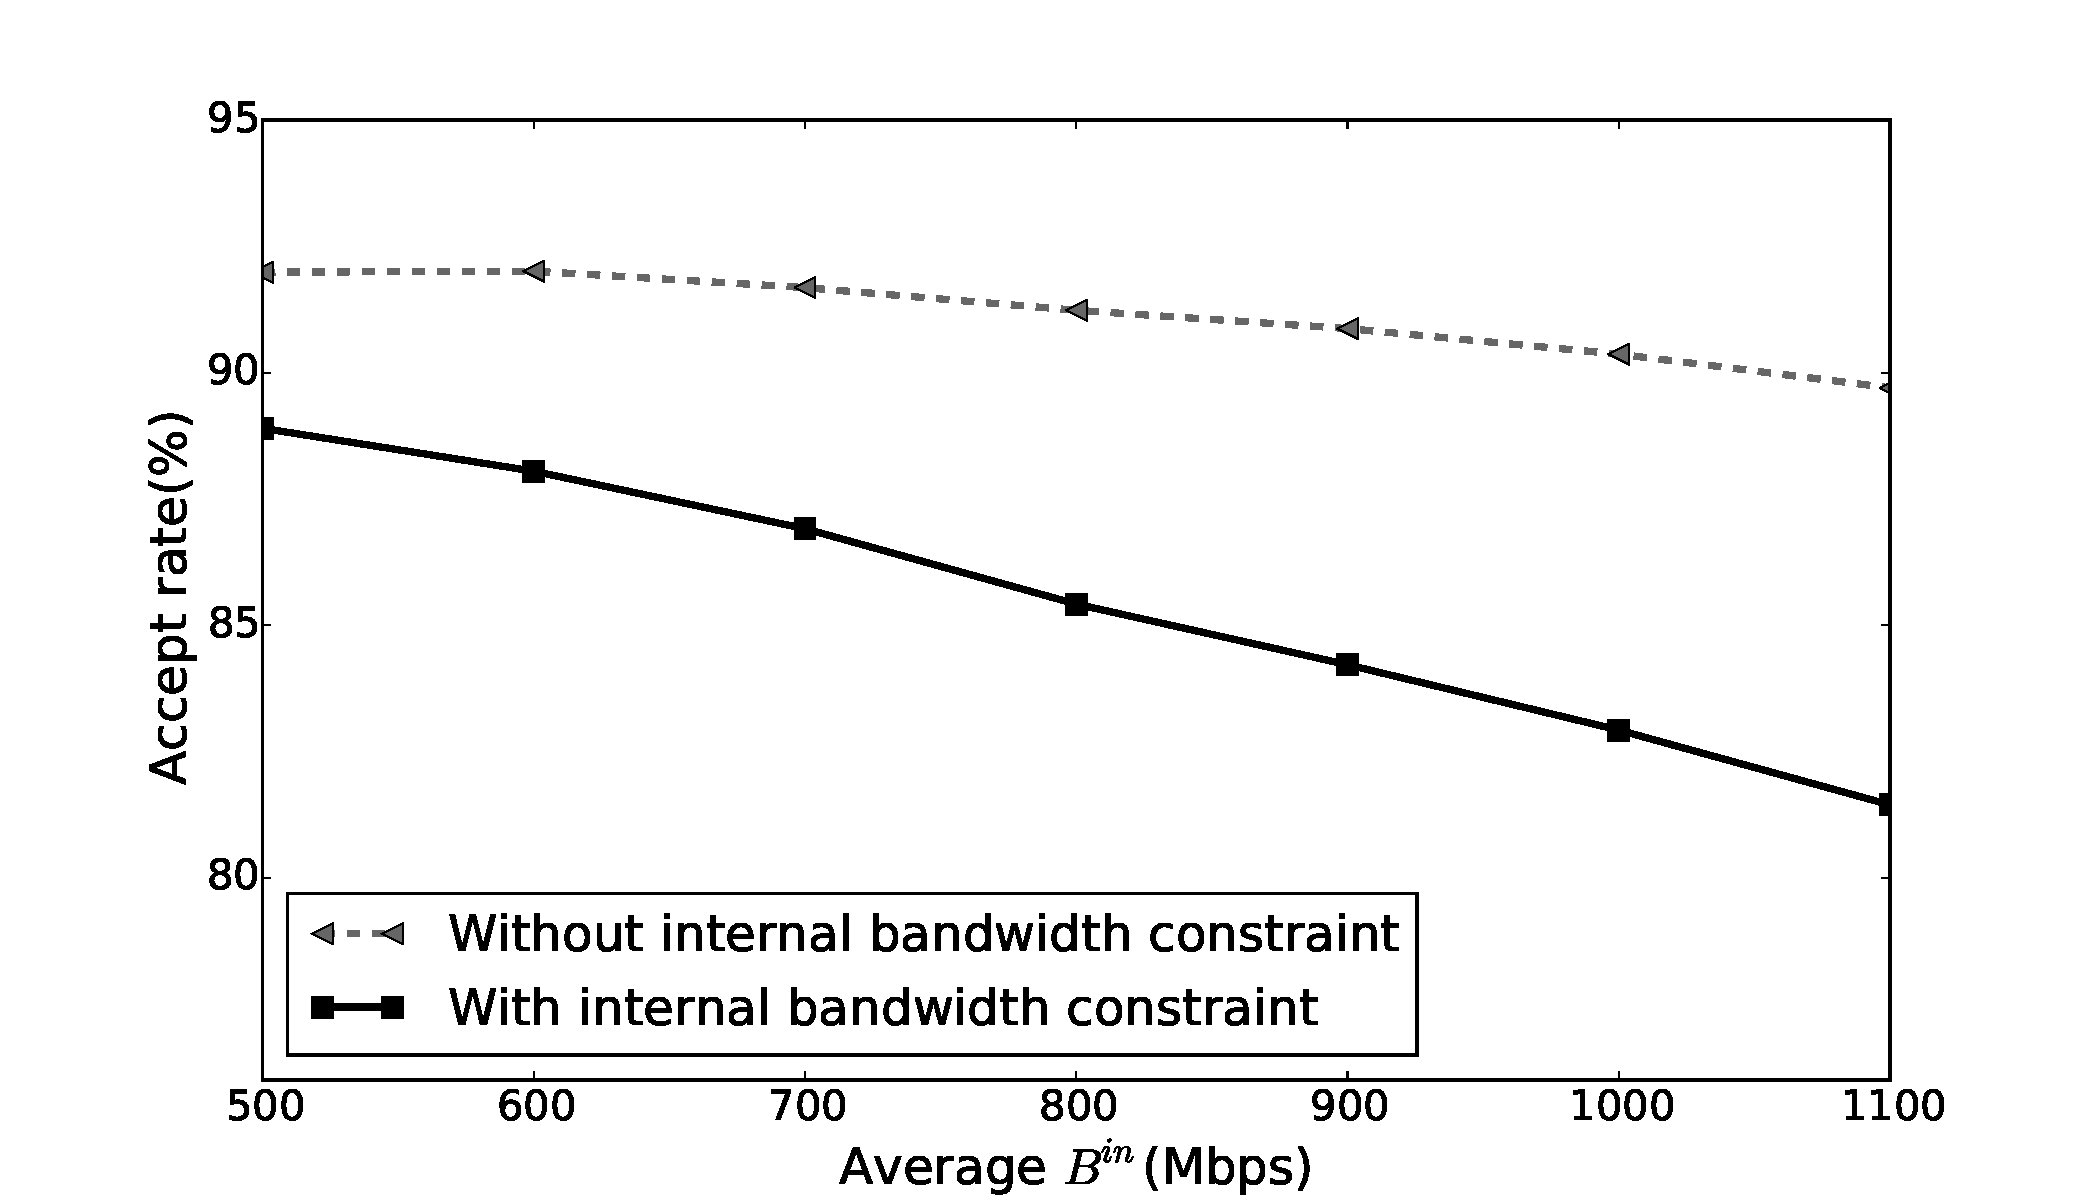
\includegraphics[width=2.8 in]{fig/Constraint.pdf}
    \caption{Accept rate with or without internal bandwidth constraint}
    \label{fig:constr}
\end{figure}

Note that the accept rate of the scenario that includes internal bandwidth constraint drops much faster than the one without the constraint. As discussed before, the max flow of inter PM traffic is calculated in a different way with upper links. The upper links are organized in a tree-like topology while the internal PM link is organized in a bus topology. The maximum flow of the tree topology is the minimum one between the left part of the link and the right part of the link, while the maximum flow of the bus topology is the max situation of the tree topology. As the link capacity and internal constraint are the same in our simulation, a request is always limited by the internal PM constraint first, which reduces the number of available VM slots and leads to lower accept rate.

\begin{figure}
\center
		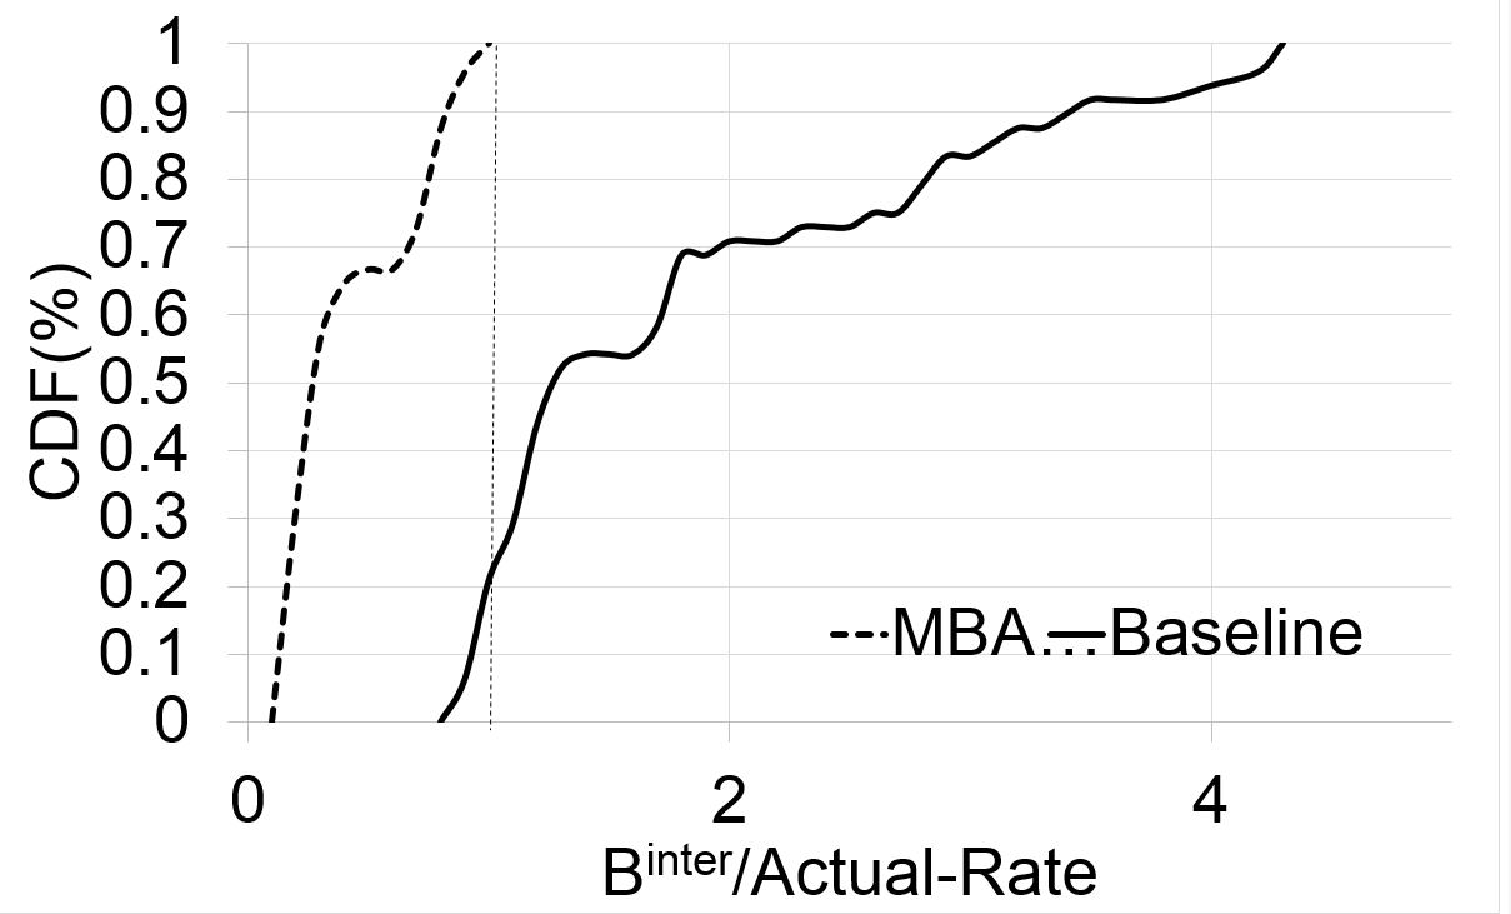
\includegraphics[width=2.8in]{fig/sim.pdf}
	\caption{Flow completion time in MBA-enabled network and baseline network}
	\label{fig:wang}
\end{figure}

It is noteworthy that the current datacenter network applies hardware middleboxes which are shared among all the tenant. These hardware middleboxes are usually attached on the switches, like FW on the core switch, IPS on the aggregation switches and LB on the ToR switch. Therefore, the inter-tenant traffic has to go to the core switches, aggregation switches and ToR before coming to the targeted tenants. Consider the scenario based on current hardware middleboxes as baseline, we evaluate the performance of software middleboxes application with MISSILE (MBA) in terms of the flow completion time with randomly generated inter-tenant traffic that satisfies the tenant's request. From Fig. \ref{fig:wang}, we can see that the flow can always complete within normalised time, since we provide minimum bandwidth guarantee through the VMs placement. However, the baseline may take 4x longer since the congestion happens on the oversubscription links. 

\section{Conclusion}\label{sec:final}
Since middleboxes are widely used in current networks, it is essential to consider middleboxes when embedding predicable virtual networks. This paper tries to fill the gap. To achieve this goal, we first model the tenant's requirement of software middleboxes and applications. By augumenting software middleboxes as VMs in the Tenant Application Graph, an VMs placement algorithm, called MISSILE, is proposed to place these VMs (including both normal application VMs and virtual middleboxes) in the underlying infrastructure. The evaluation results have shown that the proposed virtual middleboxes placement algorithm can effectively use the resource of multi-tenant datacenters and provide performance guarantee for tenants.   

 


%Abstraction can truely reflect the characteristic of tenant requirement
%The abstraction can map to the physical environment to satisfy the requirement but reduce the consumption of resources. 


%\section*{Acknowledgment}
%The authors thank anonymous reviewers for the work and constructive comments and suggestions. 


\bibliographystyle{IEEEtran}
\bibliography{reference}

\appendix
To address the problem of unpredictable MB performance, instead of allocating new resources of VMs and network after MBs are placed in datacenters, we introduce a probability model to represent the variable resource requirement of individual tenant. Through statistically multiplexing on VMs, we are able to balance the physical resources consumption and scalability requirement of software MBs. 

%To deal with scalability issue of software middleboxes with minimum bandwidth guarantee, 
We re-examine the MBs request and take the time-varying resource requirements of MBs into consideration. Specifically, the MBs' requirement is composed of a basic requirement and a variable requirement with probablity. Based on this model, we replace the $\langle T, M \rangle$ in Section \ref{sec:modelformb} with tuples $\langle T, M, m, P\rangle$, where $T$ and $M$  denote the type of MBs and the corresponding number of VMs in the basic requirement, and $m$ denotes the number of VMs in the variable subrequirement with probability $P$. For example, given $T=\{\text{FW, IDS, LB}\}, M=\{ 2, 4, 2\}, m=\{1, 2, 1\}, P=\{0.3, 0.2, 0.3\}$, we then know that the tenant requests for 2 firewall MBs and the request may increase to $2+1=3$ MBs with probability of 0.2. Similarly, 4 IDS MBs (resp. 2 LB MBs) are needed with probability of 0.8 (resp. 0.7) and 6 IDS MBs (resp. 3 LB MBs) with a probability of 0.2 (resp. 0.3). In summary, a tenant's request can be specified by multiple virtual networks (VNs) and each VN can be specified by an eight-tuple $<N, B^{in}, B^{ex}, dependencies, T, M, m, P>$. It allows elasticity by having a probability model for the number of MBs needed in each VN. 

If multiple units of subrequirement do not occur simultaneously, we can provide few redundancy to tradeoff between utilization and availability. By sharing free VMs between variable subrequirements, a specific MB can be soon deployed on the free VM once the scale up/out requirement comes. Although the subrequirement occurs with a probability less than 1, the collision may happen if there is not enough VM provided. To guarantee the performance, we apply the probabilistic model to solve this problem. For simplicity, we reuse the notation $M$ to indicate how many types of MBs are required by tenant. Let $X_{i}$ indicate whether the $i$-th subrequirement occurs. Assuming the resource requirement of different middleboxes are independent, the probability of the collision happening on one supplement VM is
\begin{align}
&Pr\left[ \sum_{i=1}^{M} X_{i} > 1 \right] & \nonumber \\
&= 1-\prod_{i=1}^{M}(1-p_{i})-\sum_{i=1}^{M}\left(p_{i}\prod_{k\in[1,M], k\neq i}(1-p_{k})\right)&
\end{align}
By providing enough number of free VMs during virtual middleboxes network deployment, the probability of collision can be guaranteed less than a collision threshold $\rho$ when the system is on board. The number of subrequirement $v$ can be determined by solving the following function:
\begin{equation}\label{equ:collision}  
		Pr\left[ \sum_{i=1}^{M} X_{i} \leq v \right] \leq \rho
\end{equation}
The collision probability $Pr\left[ \sum_{i=1}^{M} X_{i} \leq v \right]$ can be achieved based on the including excluding principle. Therefore, the total number of MB VMs to be allocated for one tenant is $|M|+v$, where $|M|$ is the number of basic MBs requirement and $v$ is the additional free VMs to be allocated as backup resources. 

\begin{figure}
	\centering
		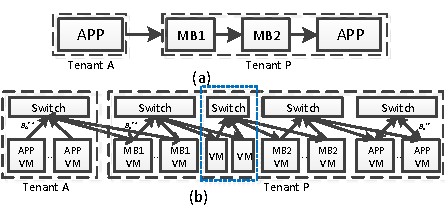
\includegraphics[width=3.3 in]{fig/scalability.pdf}
	\caption{Virtual Network Model. (a) the communication between two tenants; (b) cascade of TAG}
	\label{fig:scalability}
\end{figure}

Fig. \ref{fig:scalability} (b) uses the cascade of TAG model to abstract the communication dependency of VNs given in Fig. \ref{fig:scalability} (a). In comparison with Fig. \ref{fig:abstraction}, the VMs inside the blue dotted line are pre-allocated VMs for middleboxes subrequirement, which are shared by both types of middleboxes requests. If there are scale-out or failover request, specified MBs will be placed on these VMs to provide performance guarantee. If a tenant requires for multiple types of MBs, we can place free slots between cascade two types of MBs according to the expectation of their scalability. 

% that's all folks
\end{document}


